\documentclass[twoside]{book}

% Packages required by doxygen
\usepackage{fixltx2e}
\usepackage{calc}
\usepackage{doxygen}
\usepackage[export]{adjustbox} % also loads graphicx
\usepackage{graphicx}
\usepackage[utf8]{inputenc}
\usepackage{makeidx}
\usepackage{multicol}
\usepackage{multirow}
\PassOptionsToPackage{warn}{textcomp}
\usepackage{textcomp}
\usepackage[nointegrals]{wasysym}
\usepackage[table]{xcolor}

% Font selection
\usepackage[T1]{fontenc}
\usepackage[scaled=.90]{helvet}
\usepackage{courier}
\usepackage{amssymb}
\usepackage{sectsty}
\renewcommand{\familydefault}{\sfdefault}
\allsectionsfont{%
  \fontseries{bc}\selectfont%
  \color{darkgray}%
}
\renewcommand{\DoxyLabelFont}{%
  \fontseries{bc}\selectfont%
  \color{darkgray}%
}
\newcommand{\+}{\discretionary{\mbox{\scriptsize$\hookleftarrow$}}{}{}}

% Page & text layout
\usepackage{geometry}
\geometry{%
  a4paper,%
  top=2.5cm,%
  bottom=2.5cm,%
  left=2.5cm,%
  right=2.5cm%
}
\tolerance=750
\hfuzz=15pt
\hbadness=750
\setlength{\emergencystretch}{15pt}
\setlength{\parindent}{0cm}
\setlength{\parskip}{3ex plus 2ex minus 2ex}
\makeatletter
\renewcommand{\paragraph}{%
  \@startsection{paragraph}{4}{0ex}{-1.0ex}{1.0ex}{%
    \normalfont\normalsize\bfseries\SS@parafont%
  }%
}
\renewcommand{\subparagraph}{%
  \@startsection{subparagraph}{5}{0ex}{-1.0ex}{1.0ex}{%
    \normalfont\normalsize\bfseries\SS@subparafont%
  }%
}
\makeatother

% Headers & footers
\usepackage{fancyhdr}
\pagestyle{fancyplain}
\fancyhead[LE]{\fancyplain{}{\bfseries\thepage}}
\fancyhead[CE]{\fancyplain{}{}}
\fancyhead[RE]{\fancyplain{}{\bfseries\leftmark}}
\fancyhead[LO]{\fancyplain{}{\bfseries\rightmark}}
\fancyhead[CO]{\fancyplain{}{}}
\fancyhead[RO]{\fancyplain{}{\bfseries\thepage}}
\fancyfoot[LE]{\fancyplain{}{}}
\fancyfoot[CE]{\fancyplain{}{}}
\fancyfoot[RE]{\fancyplain{}{\bfseries\scriptsize Generated by Doxygen }}
\fancyfoot[LO]{\fancyplain{}{\bfseries\scriptsize Generated by Doxygen }}
\fancyfoot[CO]{\fancyplain{}{}}
\fancyfoot[RO]{\fancyplain{}{}}
\renewcommand{\footrulewidth}{0.4pt}
\renewcommand{\chaptermark}[1]{%
  \markboth{#1}{}%
}
\renewcommand{\sectionmark}[1]{%
  \markright{\thesection\ #1}%
}

% Indices & bibliography
\usepackage{natbib}
\usepackage[titles]{tocloft}
\setcounter{tocdepth}{3}
\setcounter{secnumdepth}{5}
\makeindex

% Hyperlinks (required, but should be loaded last)
\usepackage{ifpdf}
\ifpdf
  \usepackage[pdftex,pagebackref=true]{hyperref}
\else
  \usepackage[ps2pdf,pagebackref=true]{hyperref}
\fi
\hypersetup{%
  colorlinks=true,%
  linkcolor=blue,%
  citecolor=blue,%
  unicode%
}

% Custom commands
\newcommand{\clearemptydoublepage}{%
  \newpage{\pagestyle{empty}\cleardoublepage}%
}

\usepackage{caption}
\captionsetup{labelsep=space,justification=centering,font={bf},singlelinecheck=off,skip=4pt,position=top}

%===== C O N T E N T S =====

\begin{document}

% Titlepage & ToC
\hypersetup{pageanchor=false,
             bookmarksnumbered=true,
             pdfencoding=unicode
            }
\pagenumbering{alph}
\begin{titlepage}
\vspace*{7cm}
\begin{center}%
{\Large My Project }\\
\vspace*{1cm}
{\large Generated by Doxygen 1.8.13}\\
\end{center}
\end{titlepage}
\clearemptydoublepage
\pagenumbering{roman}
\tableofcontents
\clearemptydoublepage
\pagenumbering{arabic}
\hypersetup{pageanchor=true}

%--- Begin generated contents ---
\chapter{Hierarchical Index}
\section{Class Hierarchy}
This inheritance list is sorted roughly, but not completely, alphabetically\+:\begin{DoxyCompactList}
\item \contentsline{section}{Address\+Info}{\pageref{classAddressInfo}}{}
\item \contentsline{section}{Loop\+Tree}{\pageref{classLoopTree}}{}
\item \contentsline{section}{Loop\+Tree\+Node}{\pageref{classLoopTreeNode}}{}
\item Serialisable\+Attribute\begin{DoxyCompactList}
\item \contentsline{section}{Address\+Attribute}{\pageref{classAddressAttribute}}{}
\item \contentsline{section}{A\+R\+M\+Words\+Attribute}{\pageref{classARMWordsAttribute}}{}
\item \contentsline{section}{Meta\+Instruction\+Attribute}{\pageref{classMetaInstructionAttribute}}{}
\item \contentsline{section}{Symbol\+Table\+Attribute}{\pageref{classSymbolTableAttribute}}{}
\end{DoxyCompactList}
\item \contentsline{section}{triplet}{\pageref{classtriplet}}{}
\end{DoxyCompactList}

\chapter{Class Index}
\section{Class List}
Here are the classes, structs, unions and interfaces with brief descriptions\+:\begin{DoxyCompactList}
\item\contentsline{section}{\hyperlink{classAdd}{Add} }{\pageref{classAdd}}{}
\item\contentsline{section}{\hyperlink{classAddiu}{Addiu} }{\pageref{classAddiu}}{}
\item\contentsline{section}{\hyperlink{classAddr}{Addr} }{\pageref{classAddr}}{}
\item\contentsline{section}{\hyperlink{classArch}{Arch} }{\pageref{classArch}}{}
\item\contentsline{section}{\hyperlink{classArch__dep}{Arch\+\_\+dep} }{\pageref{classArch__dep}}{}
\item\contentsline{section}{\hyperlink{classARM}{A\+RM} }{\pageref{classARM}}{}
\item\contentsline{section}{\hyperlink{classARM__ADD}{A\+R\+M\+\_\+\+A\+DD} }{\pageref{classARM__ADD}}{}
\item\contentsline{section}{\hyperlink{classARM__BRANCH}{A\+R\+M\+\_\+\+B\+R\+A\+N\+CH} }{\pageref{classARM__BRANCH}}{}
\item\contentsline{section}{\hyperlink{classARM__COMMON}{A\+R\+M\+\_\+\+C\+O\+M\+M\+ON} }{\pageref{classARM__COMMON}}{}
\item\contentsline{section}{\hyperlink{classARM__COMPARE}{A\+R\+M\+\_\+\+C\+O\+M\+P\+A\+RE} }{\pageref{classARM__COMPARE}}{}
\item\contentsline{section}{\hyperlink{classARM__LOAD}{A\+R\+M\+\_\+\+L\+O\+AD} }{\pageref{classARM__LOAD}}{}
\item\contentsline{section}{\hyperlink{classARM__LOAD__MULTIPLE}{A\+R\+M\+\_\+\+L\+O\+A\+D\+\_\+\+M\+U\+L\+T\+I\+P\+LE} }{\pageref{classARM__LOAD__MULTIPLE}}{}
\item\contentsline{section}{\hyperlink{classARM__LOGICAL}{A\+R\+M\+\_\+\+L\+O\+G\+I\+C\+AL} }{\pageref{classARM__LOGICAL}}{}
\item\contentsline{section}{\hyperlink{classARM__MOV}{A\+R\+M\+\_\+\+M\+OV} }{\pageref{classARM__MOV}}{}
\item\contentsline{section}{\hyperlink{classARM__MUL}{A\+R\+M\+\_\+\+M\+UL} }{\pageref{classARM__MUL}}{}
\item\contentsline{section}{\hyperlink{classARM__NOP}{A\+R\+M\+\_\+\+N\+OP} }{\pageref{classARM__NOP}}{}
\item\contentsline{section}{\hyperlink{classARM__POP}{A\+R\+M\+\_\+\+P\+OP} }{\pageref{classARM__POP}}{}
\item\contentsline{section}{\hyperlink{classARM__PUSH}{A\+R\+M\+\_\+\+P\+U\+SH} }{\pageref{classARM__PUSH}}{}
\item\contentsline{section}{\hyperlink{classARM__REVERSE__SUB}{A\+R\+M\+\_\+\+R\+E\+V\+E\+R\+S\+E\+\_\+\+S\+UB} }{\pageref{classARM__REVERSE__SUB}}{}
\item\contentsline{section}{\hyperlink{classARM__SHIFT}{A\+R\+M\+\_\+\+S\+H\+I\+FT} }{\pageref{classARM__SHIFT}}{}
\item\contentsline{section}{\hyperlink{classARM__STORE}{A\+R\+M\+\_\+\+S\+T\+O\+RE} }{\pageref{classARM__STORE}}{}
\item\contentsline{section}{\hyperlink{classARM__STORE__MULTIPLE}{A\+R\+M\+\_\+\+S\+T\+O\+R\+E\+\_\+\+M\+U\+L\+T\+I\+P\+LE} }{\pageref{classARM__STORE__MULTIPLE}}{}
\item\contentsline{section}{\hyperlink{classARM__SUBTRACT}{A\+R\+M\+\_\+\+S\+U\+B\+T\+R\+A\+CT} }{\pageref{classARM__SUBTRACT}}{}
\item\contentsline{section}{\hyperlink{classARM__TODO__LOIC}{A\+R\+M\+\_\+\+T\+O\+D\+O\+\_\+\+L\+O\+IC} }{\pageref{classARM__TODO__LOIC}}{}
\item\contentsline{section}{\hyperlink{classBasic}{Basic} }{\pageref{classBasic}}{}
\item\contentsline{section}{\hyperlink{classCall}{Call} }{\pageref{classCall}}{}
\item\contentsline{section}{\hyperlink{classConditionalJump}{Conditional\+Jump} }{\pageref{classConditionalJump}}{}
\item\contentsline{section}{\hyperlink{classDAAInstruction}{D\+A\+A\+Instruction} }{\pageref{classDAAInstruction}}{}
\item\contentsline{section}{\hyperlink{classDCall}{D\+Call} }{\pageref{classDCall}}{}
\item\contentsline{section}{\hyperlink{classDLoad}{D\+Load} }{\pageref{classDLoad}}{}
\item\contentsline{section}{\hyperlink{classDStore}{D\+Store} }{\pageref{classDStore}}{}
\item\contentsline{section}{\hyperlink{classEmpty}{Empty} }{\pageref{classEmpty}}{}
\item\contentsline{section}{\hyperlink{classHex}{Hex} }{\pageref{classHex}}{}
\item\contentsline{section}{\hyperlink{classInstructionFormat}{Instruction\+Format} }{\pageref{classInstructionFormat}}{}
\item\contentsline{section}{\hyperlink{classInstructionType}{Instruction\+Type} }{\pageref{classInstructionType}}{}
\item\contentsline{section}{\hyperlink{classKillOp1}{Kill\+Op1} }{\pageref{classKillOp1}}{}
\item\contentsline{section}{\hyperlink{classKillOp2}{Kill\+Op2} }{\pageref{classKillOp2}}{}
\item\contentsline{section}{\hyperlink{classLi}{Li} }{\pageref{classLi}}{}
\item\contentsline{section}{\hyperlink{classLoad}{Load} }{\pageref{classLoad}}{}
\item\contentsline{section}{\hyperlink{classLui}{Lui} }{\pageref{classLui}}{}
\item\contentsline{section}{\hyperlink{classMIPS}{M\+I\+PS} }{\pageref{classMIPS}}{}
\item\contentsline{section}{\hyperlink{classMove}{Move} }{\pageref{classMove}}{}
\item\contentsline{section}{\hyperlink{classNop}{Nop} }{\pageref{classNop}}{}
\item\contentsline{section}{\hyperlink{classObjdumpFunction}{Objdump\+Function} }{\pageref{classObjdumpFunction}}{}
\item\contentsline{section}{\hyperlink{classObjdumpInstruction}{Objdump\+Instruction} }{\pageref{classObjdumpInstruction}}{}
\item\contentsline{section}{\hyperlink{classObjdumpSection}{Objdump\+Section} }{\pageref{classObjdumpSection}}{}
\item\contentsline{section}{\hyperlink{classObjdumpSymbolTable}{Objdump\+Symbol\+Table} }{\pageref{classObjdumpSymbolTable}}{}
\item\contentsline{section}{\hyperlink{classObjdumpVariable}{Objdump\+Variable} }{\pageref{classObjdumpVariable}}{}
\item\contentsline{section}{\hyperlink{classObjdumpWord}{Objdump\+Word} }{\pageref{classObjdumpWord}}{}
\item\contentsline{section}{\hyperlink{classPredicatedBasic}{Predicated\+Basic} }{\pageref{classPredicatedBasic}}{}
\item\contentsline{section}{\hyperlink{classPredicatedLoad}{Predicated\+Load} }{\pageref{classPredicatedLoad}}{}
\item\contentsline{section}{\hyperlink{classPredicatedStore}{Predicated\+Store} }{\pageref{classPredicatedStore}}{}
\item\contentsline{section}{\hyperlink{classrd}{rd} }{\pageref{classrd}}{}
\item\contentsline{section}{\hyperlink{classrd__hex}{rd\+\_\+hex} }{\pageref{classrd__hex}}{}
\item\contentsline{section}{\hyperlink{classrd__int}{rd\+\_\+int} }{\pageref{classrd__int}}{}
\item\contentsline{section}{\hyperlink{classrd__mem}{rd\+\_\+mem} }{\pageref{classrd__mem}}{}
\item\contentsline{section}{\hyperlink{classrd__mem__int}{rd\+\_\+mem\+\_\+int} }{\pageref{classrd__mem__int}}{}
\item\contentsline{section}{\hyperlink{classrd__mem__rs}{rd\+\_\+mem\+\_\+rs} }{\pageref{classrd__mem__rs}}{}
\item\contentsline{section}{\hyperlink{classrd__mem__rs__shifter}{rd\+\_\+mem\+\_\+rs\+\_\+shifter} }{\pageref{classrd__mem__rs__shifter}}{}
\item\contentsline{section}{\hyperlink{classrd__rd__rs__rs}{rd\+\_\+rd\+\_\+rs\+\_\+rs} }{\pageref{classrd__rd__rs__rs}}{}
\item\contentsline{section}{\hyperlink{classrd__rs}{rd\+\_\+rs} }{\pageref{classrd__rs}}{}
\item\contentsline{section}{\hyperlink{classrd__rs__hex}{rd\+\_\+rs\+\_\+hex} }{\pageref{classrd__rs__hex}}{}
\item\contentsline{section}{\hyperlink{classrd__rs__int}{rd\+\_\+rs\+\_\+int} }{\pageref{classrd__rs__int}}{}
\item\contentsline{section}{\hyperlink{classrd__rs__rs}{rd\+\_\+rs\+\_\+rs} }{\pageref{classrd__rs__rs}}{}
\item\contentsline{section}{\hyperlink{classrd__rs__rs__rs}{rd\+\_\+rs\+\_\+rs\+\_\+rs} }{\pageref{classrd__rs__rs__rs}}{}
\item\contentsline{section}{\hyperlink{classrd__rs__rs__shifter}{rd\+\_\+rs\+\_\+rs\+\_\+shifter} }{\pageref{classrd__rs__rs__shifter}}{}
\item\contentsline{section}{\hyperlink{classrd__rs__shifter}{rd\+\_\+rs\+\_\+shifter} }{\pageref{classrd__rs__shifter}}{}
\item\contentsline{section}{\hyperlink{classrdlist}{rdlist} }{\pageref{classrdlist}}{}
\item\contentsline{section}{\hyperlink{classrds__hex}{rds\+\_\+hex} }{\pageref{classrds__hex}}{}
\item\contentsline{section}{\hyperlink{classrds__int}{rds\+\_\+int} }{\pageref{classrds__int}}{}
\item\contentsline{section}{\hyperlink{classrds__rdlist}{rds\+\_\+rdlist} }{\pageref{classrds__rdlist}}{}
\item\contentsline{section}{\hyperlink{classrds__rds__rs__rs}{rds\+\_\+rds\+\_\+rs\+\_\+rs} }{\pageref{classrds__rds__rs__rs}}{}
\item\contentsline{section}{\hyperlink{classrds__rslist}{rds\+\_\+rslist} }{\pageref{classrds__rslist}}{}
\item\contentsline{section}{\hyperlink{classReturn}{Return} }{\pageref{classReturn}}{}
\item\contentsline{section}{\hyperlink{classrs}{rs} }{\pageref{classrs}}{}
\item\contentsline{section}{\hyperlink{classrs__addr}{rs\+\_\+addr} }{\pageref{classrs__addr}}{}
\item\contentsline{section}{\hyperlink{classrs__hex}{rs\+\_\+hex} }{\pageref{classrs__hex}}{}
\item\contentsline{section}{\hyperlink{classrs__int}{rs\+\_\+int} }{\pageref{classrs__int}}{}
\item\contentsline{section}{\hyperlink{classrs__mem}{rs\+\_\+mem} }{\pageref{classrs__mem}}{}
\item\contentsline{section}{\hyperlink{classrs__mem__int}{rs\+\_\+mem\+\_\+int} }{\pageref{classrs__mem__int}}{}
\item\contentsline{section}{\hyperlink{classrs__mem__rs}{rs\+\_\+mem\+\_\+rs} }{\pageref{classrs__mem__rs}}{}
\item\contentsline{section}{\hyperlink{classrs__mem__rs__shifter}{rs\+\_\+mem\+\_\+rs\+\_\+shifter} }{\pageref{classrs__mem__rs__shifter}}{}
\item\contentsline{section}{\hyperlink{classrs__rd}{rs\+\_\+rd} }{\pageref{classrs__rd}}{}
\item\contentsline{section}{\hyperlink{classrs__rdlist}{rs\+\_\+rdlist} }{\pageref{classrs__rdlist}}{}
\item\contentsline{section}{\hyperlink{classrs__rs}{rs\+\_\+rs} }{\pageref{classrs__rs}}{}
\item\contentsline{section}{\hyperlink{classrs__rs__addr}{rs\+\_\+rs\+\_\+addr} }{\pageref{classrs__rs__addr}}{}
\item\contentsline{section}{\hyperlink{classrs__rs__shifter}{rs\+\_\+rs\+\_\+shifter} }{\pageref{classrs__rs__shifter}}{}
\item\contentsline{section}{\hyperlink{classrs__rslist}{rs\+\_\+rslist} }{\pageref{classrs__rslist}}{}
\item\contentsline{section}{\hyperlink{classrs__zero__hex}{rs\+\_\+zero\+\_\+hex} }{\pageref{classrs__zero__hex}}{}
\item\contentsline{section}{\hyperlink{classrslist}{rslist} }{\pageref{classrslist}}{}
\item\contentsline{section}{\hyperlink{classShift}{Shift} }{\pageref{classShift}}{}
\item\contentsline{section}{\hyperlink{classStore}{Store} }{\pageref{classStore}}{}
\item\contentsline{section}{\hyperlink{classSubu}{Subu} }{\pageref{classSubu}}{}
\item\contentsline{section}{\hyperlink{classUnconditionalJump}{Unconditional\+Jump} }{\pageref{classUnconditionalJump}}{}
\item\contentsline{section}{\hyperlink{classWord}{Word} }{\pageref{classWord}}{}
\item\contentsline{section}{\hyperlink{classzero__rs__rs}{zero\+\_\+rs\+\_\+rs} }{\pageref{classzero__rs__rs}}{}
\end{DoxyCompactList}

\chapter{File Index}
\section{File List}
Here is a list of all files with brief descriptions\+:\begin{DoxyCompactList}
\item\contentsline{section}{src/\hyperlink{HeptaneStdTypes_8h}{Heptane\+Std\+Types.\+h} }{\pageref{HeptaneStdTypes_8h}}{}
\item\contentsline{section}{src/\hyperlink{InstructionARM_8h}{Instruction\+A\+R\+M.\+h} }{\pageref{InstructionARM_8h}}{}
\item\contentsline{section}{src/\hyperlink{Logger_8h}{Logger.\+h} }{\pageref{Logger_8h}}{}
\item\contentsline{section}{src/\hyperlink{Utl_8h}{Utl.\+h} }{\pageref{Utl_8h}}{}
\end{DoxyCompactList}

\chapter{Class Documentation}
\hypertarget{classAddressAttribute}{}\section{Address\+Attribute Class Reference}
\label{classAddressAttribute}\index{Address\+Attribute@{Address\+Attribute}}


{\ttfamily \#include $<$Address\+Attribute.\+h$>$}

Inheritance diagram for Address\+Attribute\+:\begin{figure}[H]
\begin{center}
\leavevmode
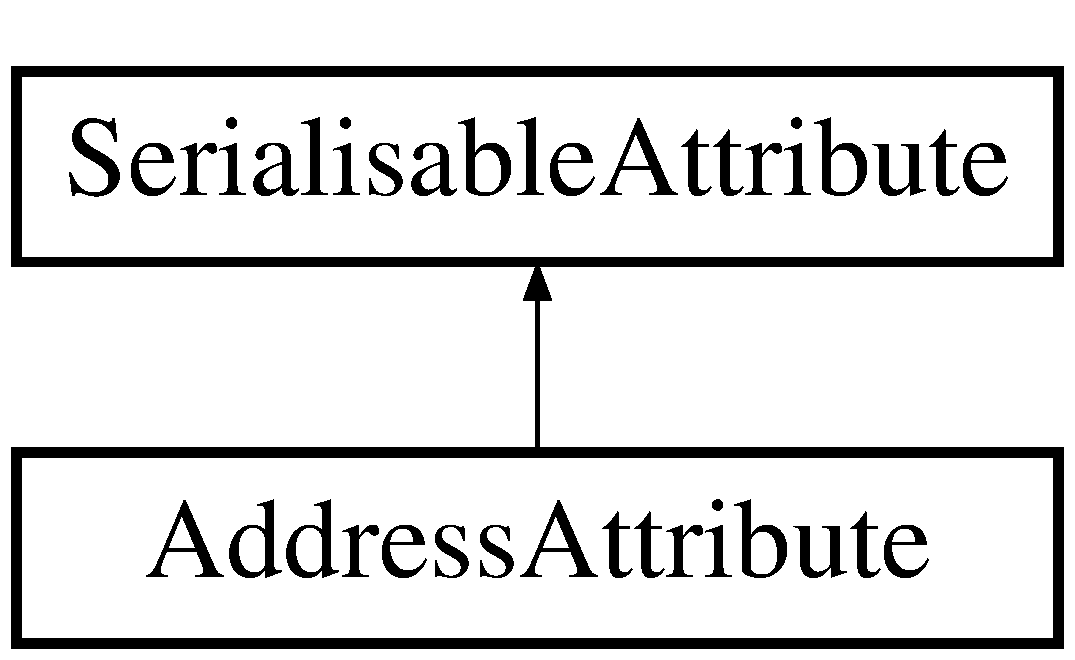
\includegraphics[height=2.000000cm]{classAddressAttribute}
\end{center}
\end{figure}
\subsection*{Public Member Functions}
\begin{DoxyCompactItemize}
\item 
\hyperlink{classAddressAttribute_ace33470ed7a894142633a223b64378af}{Address\+Attribute} ()
\item 
vector$<$ \hyperlink{classAddressInfo}{Address\+Info} $>$ \hyperlink{classAddressAttribute_ac7c1a2d8160f4db5423fd53dc305f886}{get\+List\+Info} ()
\item 
\hyperlink{classAddressAttribute}{Address\+Attribute} $\ast$ \hyperlink{classAddressAttribute_ab418a5c40c38661892b790274dac50a0}{clone} ()
\item 
ostream \& \hyperlink{classAddressAttribute_ad189a02a8d2bc9058cd35bebf3f1210f}{Write\+Xml} (std\+::ostream \&, cfglib\+::\+Handle \&)
\item 
void \hyperlink{classAddressAttribute_a08871197b24a886864a337896ebab051}{Read\+Xml} (Xml\+Tag const $\ast$xml\+\_\+node, cfglib\+::\+Handle \&)
\item 
void \hyperlink{classAddressAttribute_aaa60489ef43cad77278ef19325dcd18c}{add\+Info} (\hyperlink{classAddressInfo}{Address\+Info})
\item 
long \hyperlink{classAddressAttribute_afebe2c5206d6e06ff5e479433a299ffa}{get\+Code\+Address} ()
\item 
Serialisable\+Attribute $\ast$ \hyperlink{classAddressAttribute_a25b4e25c9284dcdea23b761ca519dcd8}{create} ()
\item 
void \hyperlink{classAddressAttribute_a862ec35a0100f0486d466eac3cdb1cc3}{Print} (std\+::ostream \&)
\end{DoxyCompactItemize}


\subsection{Detailed Description}
The Address attribute class

This attribute is generate by the M\+I\+P\+S\+Address\+Analysis and is attached to each asm instruction of a program 

\subsection{Constructor \& Destructor Documentation}
\mbox{\Hypertarget{classAddressAttribute_ace33470ed7a894142633a223b64378af}\label{classAddressAttribute_ace33470ed7a894142633a223b64378af}} 
\index{Address\+Attribute@{Address\+Attribute}!Address\+Attribute@{Address\+Attribute}}
\index{Address\+Attribute@{Address\+Attribute}!Address\+Attribute@{Address\+Attribute}}
\subsubsection{\texorpdfstring{Address\+Attribute()}{AddressAttribute()}}
{\footnotesize\ttfamily Address\+Attribute\+::\+Address\+Attribute (\begin{DoxyParamCaption}{ }\end{DoxyParamCaption})}

constructor 

\subsection{Member Function Documentation}
\mbox{\Hypertarget{classAddressAttribute_aaa60489ef43cad77278ef19325dcd18c}\label{classAddressAttribute_aaa60489ef43cad77278ef19325dcd18c}} 
\index{Address\+Attribute@{Address\+Attribute}!add\+Info@{add\+Info}}
\index{add\+Info@{add\+Info}!Address\+Attribute@{Address\+Attribute}}
\subsubsection{\texorpdfstring{add\+Info()}{addInfo()}}
{\footnotesize\ttfamily void Address\+Attribute\+::add\+Info (\begin{DoxyParamCaption}\item[{\hyperlink{classAddressInfo}{Address\+Info}}]{ }\end{DoxyParamCaption})}

This function add an object \hyperlink{classAddressInfo}{Address\+Info} to the list\+Info vector of this \mbox{\Hypertarget{classAddressAttribute_ab418a5c40c38661892b790274dac50a0}\label{classAddressAttribute_ab418a5c40c38661892b790274dac50a0}} 
\index{Address\+Attribute@{Address\+Attribute}!clone@{clone}}
\index{clone@{clone}!Address\+Attribute@{Address\+Attribute}}
\subsubsection{\texorpdfstring{clone()}{clone()}}
{\footnotesize\ttfamily \hyperlink{classAddressAttribute}{Address\+Attribute}$\ast$ Address\+Attribute\+::clone (\begin{DoxyParamCaption}{ }\end{DoxyParamCaption})}

\mbox{\Hypertarget{classAddressAttribute_a25b4e25c9284dcdea23b761ca519dcd8}\label{classAddressAttribute_a25b4e25c9284dcdea23b761ca519dcd8}} 
\index{Address\+Attribute@{Address\+Attribute}!create@{create}}
\index{create@{create}!Address\+Attribute@{Address\+Attribute}}
\subsubsection{\texorpdfstring{create()}{create()}}
{\footnotesize\ttfamily Serialisable\+Attribute$\ast$ Address\+Attribute\+::create (\begin{DoxyParamCaption}{ }\end{DoxyParamCaption})}

\mbox{\Hypertarget{classAddressAttribute_afebe2c5206d6e06ff5e479433a299ffa}\label{classAddressAttribute_afebe2c5206d6e06ff5e479433a299ffa}} 
\index{Address\+Attribute@{Address\+Attribute}!get\+Code\+Address@{get\+Code\+Address}}
\index{get\+Code\+Address@{get\+Code\+Address}!Address\+Attribute@{Address\+Attribute}}
\subsubsection{\texorpdfstring{get\+Code\+Address()}{getCodeAddress()}}
{\footnotesize\ttfamily long Address\+Attribute\+::get\+Code\+Address (\begin{DoxyParamCaption}{ }\end{DoxyParamCaption})}

return the code begin address of the code associated to the instruction or -\/1 if it is not an asm instruction \mbox{\Hypertarget{classAddressAttribute_ac7c1a2d8160f4db5423fd53dc305f886}\label{classAddressAttribute_ac7c1a2d8160f4db5423fd53dc305f886}} 
\index{Address\+Attribute@{Address\+Attribute}!get\+List\+Info@{get\+List\+Info}}
\index{get\+List\+Info@{get\+List\+Info}!Address\+Attribute@{Address\+Attribute}}
\subsubsection{\texorpdfstring{get\+List\+Info()}{getListInfo()}}
{\footnotesize\ttfamily vector$<$\hyperlink{classAddressInfo}{Address\+Info}$>$ Address\+Attribute\+::get\+List\+Info (\begin{DoxyParamCaption}{ }\end{DoxyParamCaption})}

accessor \mbox{\Hypertarget{classAddressAttribute_a862ec35a0100f0486d466eac3cdb1cc3}\label{classAddressAttribute_a862ec35a0100f0486d466eac3cdb1cc3}} 
\index{Address\+Attribute@{Address\+Attribute}!Print@{Print}}
\index{Print@{Print}!Address\+Attribute@{Address\+Attribute}}
\subsubsection{\texorpdfstring{Print()}{Print()}}
{\footnotesize\ttfamily void Address\+Attribute\+::\+Print (\begin{DoxyParamCaption}\item[{std\+::ostream \&}]{ }\end{DoxyParamCaption})}

\mbox{\Hypertarget{classAddressAttribute_a08871197b24a886864a337896ebab051}\label{classAddressAttribute_a08871197b24a886864a337896ebab051}} 
\index{Address\+Attribute@{Address\+Attribute}!Read\+Xml@{Read\+Xml}}
\index{Read\+Xml@{Read\+Xml}!Address\+Attribute@{Address\+Attribute}}
\subsubsection{\texorpdfstring{Read\+Xml()}{ReadXml()}}
{\footnotesize\ttfamily void Address\+Attribute\+::\+Read\+Xml (\begin{DoxyParamCaption}\item[{Xml\+Tag const $\ast$}]{xml\+\_\+node,  }\item[{cfglib\+::\+Handle \&}]{ }\end{DoxyParamCaption})}

\mbox{\Hypertarget{classAddressAttribute_ad189a02a8d2bc9058cd35bebf3f1210f}\label{classAddressAttribute_ad189a02a8d2bc9058cd35bebf3f1210f}} 
\index{Address\+Attribute@{Address\+Attribute}!Write\+Xml@{Write\+Xml}}
\index{Write\+Xml@{Write\+Xml}!Address\+Attribute@{Address\+Attribute}}
\subsubsection{\texorpdfstring{Write\+Xml()}{WriteXml()}}
{\footnotesize\ttfamily ostream\& Address\+Attribute\+::\+Write\+Xml (\begin{DoxyParamCaption}\item[{std\+::ostream \&}]{,  }\item[{cfglib\+::\+Handle \&}]{ }\end{DoxyParamCaption})}



The documentation for this class was generated from the following file\+:\begin{DoxyCompactItemize}
\item 
src/\hyperlink{AddressAttribute_8h}{Address\+Attribute.\+h}\end{DoxyCompactItemize}

\hypertarget{classAddressInfo}{}\section{Address\+Info Class Reference}
\label{classAddressInfo}\index{Address\+Info@{Address\+Info}}


{\ttfamily \#include $<$Address\+Attribute.\+h$>$}

\subsection*{Public Member Functions}
\begin{DoxyCompactItemize}
\item 
\hyperlink{classAddressInfo_a1d82e681b86d769de4325b99163ed640}{Address\+Info} ()
\item 
void \hyperlink{classAddressInfo_a37271fcb2207dc8b7f816907760fc721}{set\+Name} (string n)
\item 
void \hyperlink{classAddressInfo_a024ac80e1b8a35625cb77d6a4c8e6b0e}{set\+Type} (string t)
\item 
void \hyperlink{classAddressInfo_a9e530ba6525d74f46da29705a032e84c}{set\+Segment} (string seg)
\item 
void \hyperlink{classAddressInfo_a5c8bf00c9f0816ef0dc9794317434418}{set\+Precision} (bool p)
\item 
vector$<$ pair$<$ string, string $>$ $>$ \hyperlink{classAddressInfo_a459c495a6d820e9312d733a816a3ba79}{get\+Adr\+Size} ()
\item 
string \hyperlink{classAddressInfo_ad4decf39436c2c5f5c7725dd72d1c4e9}{get\+Type} ()
\item 
string \hyperlink{classAddressInfo_abe571cf9594ec7309baec30df6b5fc9a}{get\+Name} ()
\item 
string \hyperlink{classAddressInfo_a672a6460879dc1f63eb1fd8ee6d18b55}{get\+Segment} ()
\item 
bool \hyperlink{classAddressInfo_ac833d1421bef4e4f936a7bad9686c795}{get\+Precision} ()
\item 
void \hyperlink{classAddressInfo_a90a057789302f68c43f07ffaafb53af1}{add\+Adr\+Size} (string adr, string size)
\item 
void \hyperlink{classAddressInfo_a2c82626af62f839742cfa6797f257e6f}{print} ()
\end{DoxyCompactItemize}


\subsection{Detailed Description}
The class \hyperlink{classAddressInfo}{Address\+Info} is a structure to group the informations of 1 access to memory realized by an instruction 

\subsection{Constructor \& Destructor Documentation}
\mbox{\Hypertarget{classAddressInfo_a1d82e681b86d769de4325b99163ed640}\label{classAddressInfo_a1d82e681b86d769de4325b99163ed640}} 
\index{Address\+Info@{Address\+Info}!Address\+Info@{Address\+Info}}
\index{Address\+Info@{Address\+Info}!Address\+Info@{Address\+Info}}
\subsubsection{\texorpdfstring{Address\+Info()}{AddressInfo()}}
{\footnotesize\ttfamily Address\+Info\+::\+Address\+Info (\begin{DoxyParamCaption}{ }\end{DoxyParamCaption})}



\subsection{Member Function Documentation}
\mbox{\Hypertarget{classAddressInfo_a90a057789302f68c43f07ffaafb53af1}\label{classAddressInfo_a90a057789302f68c43f07ffaafb53af1}} 
\index{Address\+Info@{Address\+Info}!add\+Adr\+Size@{add\+Adr\+Size}}
\index{add\+Adr\+Size@{add\+Adr\+Size}!Address\+Info@{Address\+Info}}
\subsubsection{\texorpdfstring{add\+Adr\+Size()}{addAdrSize()}}
{\footnotesize\ttfamily void Address\+Info\+::add\+Adr\+Size (\begin{DoxyParamCaption}\item[{string}]{adr,  }\item[{string}]{size }\end{DoxyParamCaption})}

This function is used to add a pair\+: $<$begin address to memory area acceded ; size of the access in byte$>$ \mbox{\Hypertarget{classAddressInfo_a459c495a6d820e9312d733a816a3ba79}\label{classAddressInfo_a459c495a6d820e9312d733a816a3ba79}} 
\index{Address\+Info@{Address\+Info}!get\+Adr\+Size@{get\+Adr\+Size}}
\index{get\+Adr\+Size@{get\+Adr\+Size}!Address\+Info@{Address\+Info}}
\subsubsection{\texorpdfstring{get\+Adr\+Size()}{getAdrSize()}}
{\footnotesize\ttfamily vector$<$pair$<$string,string$>$ $>$ Address\+Info\+::get\+Adr\+Size (\begin{DoxyParamCaption}{ }\end{DoxyParamCaption})}

\mbox{\Hypertarget{classAddressInfo_abe571cf9594ec7309baec30df6b5fc9a}\label{classAddressInfo_abe571cf9594ec7309baec30df6b5fc9a}} 
\index{Address\+Info@{Address\+Info}!get\+Name@{get\+Name}}
\index{get\+Name@{get\+Name}!Address\+Info@{Address\+Info}}
\subsubsection{\texorpdfstring{get\+Name()}{getName()}}
{\footnotesize\ttfamily string Address\+Info\+::get\+Name (\begin{DoxyParamCaption}{ }\end{DoxyParamCaption})}

\mbox{\Hypertarget{classAddressInfo_ac833d1421bef4e4f936a7bad9686c795}\label{classAddressInfo_ac833d1421bef4e4f936a7bad9686c795}} 
\index{Address\+Info@{Address\+Info}!get\+Precision@{get\+Precision}}
\index{get\+Precision@{get\+Precision}!Address\+Info@{Address\+Info}}
\subsubsection{\texorpdfstring{get\+Precision()}{getPrecision()}}
{\footnotesize\ttfamily bool Address\+Info\+::get\+Precision (\begin{DoxyParamCaption}{ }\end{DoxyParamCaption})}

\mbox{\Hypertarget{classAddressInfo_a672a6460879dc1f63eb1fd8ee6d18b55}\label{classAddressInfo_a672a6460879dc1f63eb1fd8ee6d18b55}} 
\index{Address\+Info@{Address\+Info}!get\+Segment@{get\+Segment}}
\index{get\+Segment@{get\+Segment}!Address\+Info@{Address\+Info}}
\subsubsection{\texorpdfstring{get\+Segment()}{getSegment()}}
{\footnotesize\ttfamily string Address\+Info\+::get\+Segment (\begin{DoxyParamCaption}{ }\end{DoxyParamCaption})}

\mbox{\Hypertarget{classAddressInfo_ad4decf39436c2c5f5c7725dd72d1c4e9}\label{classAddressInfo_ad4decf39436c2c5f5c7725dd72d1c4e9}} 
\index{Address\+Info@{Address\+Info}!get\+Type@{get\+Type}}
\index{get\+Type@{get\+Type}!Address\+Info@{Address\+Info}}
\subsubsection{\texorpdfstring{get\+Type()}{getType()}}
{\footnotesize\ttfamily string Address\+Info\+::get\+Type (\begin{DoxyParamCaption}{ }\end{DoxyParamCaption})}

\mbox{\Hypertarget{classAddressInfo_a2c82626af62f839742cfa6797f257e6f}\label{classAddressInfo_a2c82626af62f839742cfa6797f257e6f}} 
\index{Address\+Info@{Address\+Info}!print@{print}}
\index{print@{print}!Address\+Info@{Address\+Info}}
\subsubsection{\texorpdfstring{print()}{print()}}
{\footnotesize\ttfamily void Address\+Info\+::print (\begin{DoxyParamCaption}{ }\end{DoxyParamCaption})}

\mbox{\Hypertarget{classAddressInfo_a37271fcb2207dc8b7f816907760fc721}\label{classAddressInfo_a37271fcb2207dc8b7f816907760fc721}} 
\index{Address\+Info@{Address\+Info}!set\+Name@{set\+Name}}
\index{set\+Name@{set\+Name}!Address\+Info@{Address\+Info}}
\subsubsection{\texorpdfstring{set\+Name()}{setName()}}
{\footnotesize\ttfamily void Address\+Info\+::set\+Name (\begin{DoxyParamCaption}\item[{string}]{n }\end{DoxyParamCaption})}

accessors \mbox{\Hypertarget{classAddressInfo_a5c8bf00c9f0816ef0dc9794317434418}\label{classAddressInfo_a5c8bf00c9f0816ef0dc9794317434418}} 
\index{Address\+Info@{Address\+Info}!set\+Precision@{set\+Precision}}
\index{set\+Precision@{set\+Precision}!Address\+Info@{Address\+Info}}
\subsubsection{\texorpdfstring{set\+Precision()}{setPrecision()}}
{\footnotesize\ttfamily void Address\+Info\+::set\+Precision (\begin{DoxyParamCaption}\item[{bool}]{p }\end{DoxyParamCaption})}

\mbox{\Hypertarget{classAddressInfo_a9e530ba6525d74f46da29705a032e84c}\label{classAddressInfo_a9e530ba6525d74f46da29705a032e84c}} 
\index{Address\+Info@{Address\+Info}!set\+Segment@{set\+Segment}}
\index{set\+Segment@{set\+Segment}!Address\+Info@{Address\+Info}}
\subsubsection{\texorpdfstring{set\+Segment()}{setSegment()}}
{\footnotesize\ttfamily void Address\+Info\+::set\+Segment (\begin{DoxyParamCaption}\item[{string}]{seg }\end{DoxyParamCaption})}

\mbox{\Hypertarget{classAddressInfo_a024ac80e1b8a35625cb77d6a4c8e6b0e}\label{classAddressInfo_a024ac80e1b8a35625cb77d6a4c8e6b0e}} 
\index{Address\+Info@{Address\+Info}!set\+Type@{set\+Type}}
\index{set\+Type@{set\+Type}!Address\+Info@{Address\+Info}}
\subsubsection{\texorpdfstring{set\+Type()}{setType()}}
{\footnotesize\ttfamily void Address\+Info\+::set\+Type (\begin{DoxyParamCaption}\item[{string}]{t }\end{DoxyParamCaption})}



The documentation for this class was generated from the following file\+:\begin{DoxyCompactItemize}
\item 
src/\hyperlink{AddressAttribute_8h}{Address\+Attribute.\+h}\end{DoxyCompactItemize}

\hypertarget{classARMWordsAttribute}{}\section{A\+R\+M\+Words\+Attribute Class Reference}
\label{classARMWordsAttribute}\index{A\+R\+M\+Words\+Attribute@{A\+R\+M\+Words\+Attribute}}


{\ttfamily \#include $<$A\+R\+M\+Words\+Attribute.\+h$>$}

Inheritance diagram for A\+R\+M\+Words\+Attribute\+:\begin{figure}[H]
\begin{center}
\leavevmode
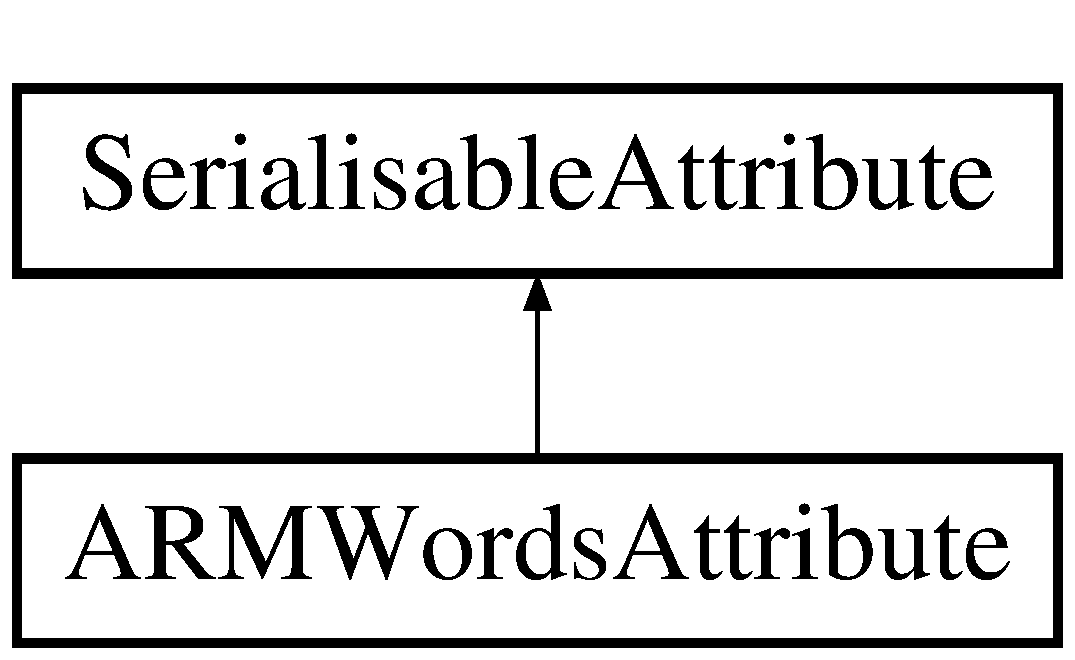
\includegraphics[height=2.000000cm]{classARMWordsAttribute}
\end{center}
\end{figure}
\subsection*{Public Member Functions}
\begin{DoxyCompactItemize}
\item 
\hyperlink{classARMWordsAttribute_a6e11470ad050e0fd7eeb7a094a543bcd}{A\+R\+M\+Words\+Attribute} ()
\item 
\hyperlink{classARMWordsAttribute}{A\+R\+M\+Words\+Attribute} $\ast$ \hyperlink{classARMWordsAttribute_af4ec429b5d88102773cc84de7d8dabcb}{clone} ()
\item 
ostream \& \hyperlink{classARMWordsAttribute_ad0061dc1aaa8a4a8264885f39798372c}{Write\+Xml} (std\+::ostream \&, cfglib\+::\+Handle \&)
\item 
void \hyperlink{classARMWordsAttribute_a661a7fbe6c6eab0a5e0c371525d92961}{Read\+Xml} (Xml\+Tag const $\ast$xml\+\_\+node, cfglib\+::\+Handle \&)
\item 
Serialisable\+Attribute $\ast$ \hyperlink{classARMWordsAttribute_a5989e2a2f17a9e9bfdcd76c0543e0720}{create} ()
\item 
void \hyperlink{classARMWordsAttribute_a6875eb117a936a45fbb6e90e3a2ecad9}{Print} (std\+::ostream \&)
\item 
void \hyperlink{classARMWordsAttribute_a9c5ac94cef5510b90dad76940413c2db}{add\+Word} (unsigned long addr, string type, unsigned long value)
\item 
\hyperlink{ARMWordsAttribute_8h_a7d589468d1898466a80161546d217fd6}{A\+R\+M\+Words\+Attribute\+Table} \hyperlink{classARMWordsAttribute_a6326d1ca018bc249d6dc28713af800a0}{get\+Table} ()
\end{DoxyCompactItemize}


\subsection{Constructor \& Destructor Documentation}
\mbox{\Hypertarget{classARMWordsAttribute_a6e11470ad050e0fd7eeb7a094a543bcd}\label{classARMWordsAttribute_a6e11470ad050e0fd7eeb7a094a543bcd}} 
\index{A\+R\+M\+Words\+Attribute@{A\+R\+M\+Words\+Attribute}!A\+R\+M\+Words\+Attribute@{A\+R\+M\+Words\+Attribute}}
\index{A\+R\+M\+Words\+Attribute@{A\+R\+M\+Words\+Attribute}!A\+R\+M\+Words\+Attribute@{A\+R\+M\+Words\+Attribute}}
\subsubsection{\texorpdfstring{A\+R\+M\+Words\+Attribute()}{ARMWordsAttribute()}}
{\footnotesize\ttfamily A\+R\+M\+Words\+Attribute\+::\+A\+R\+M\+Words\+Attribute (\begin{DoxyParamCaption}{ }\end{DoxyParamCaption})}

constructor 

\subsection{Member Function Documentation}
\mbox{\Hypertarget{classARMWordsAttribute_a9c5ac94cef5510b90dad76940413c2db}\label{classARMWordsAttribute_a9c5ac94cef5510b90dad76940413c2db}} 
\index{A\+R\+M\+Words\+Attribute@{A\+R\+M\+Words\+Attribute}!add\+Word@{add\+Word}}
\index{add\+Word@{add\+Word}!A\+R\+M\+Words\+Attribute@{A\+R\+M\+Words\+Attribute}}
\subsubsection{\texorpdfstring{add\+Word()}{addWord()}}
{\footnotesize\ttfamily void A\+R\+M\+Words\+Attribute\+::add\+Word (\begin{DoxyParamCaption}\item[{unsigned long}]{addr,  }\item[{string}]{type,  }\item[{unsigned long}]{value }\end{DoxyParamCaption})}

\mbox{\Hypertarget{classARMWordsAttribute_af4ec429b5d88102773cc84de7d8dabcb}\label{classARMWordsAttribute_af4ec429b5d88102773cc84de7d8dabcb}} 
\index{A\+R\+M\+Words\+Attribute@{A\+R\+M\+Words\+Attribute}!clone@{clone}}
\index{clone@{clone}!A\+R\+M\+Words\+Attribute@{A\+R\+M\+Words\+Attribute}}
\subsubsection{\texorpdfstring{clone()}{clone()}}
{\footnotesize\ttfamily \hyperlink{classARMWordsAttribute}{A\+R\+M\+Words\+Attribute}$\ast$ A\+R\+M\+Words\+Attribute\+::clone (\begin{DoxyParamCaption}{ }\end{DoxyParamCaption})}

cloning function \mbox{\Hypertarget{classARMWordsAttribute_a5989e2a2f17a9e9bfdcd76c0543e0720}\label{classARMWordsAttribute_a5989e2a2f17a9e9bfdcd76c0543e0720}} 
\index{A\+R\+M\+Words\+Attribute@{A\+R\+M\+Words\+Attribute}!create@{create}}
\index{create@{create}!A\+R\+M\+Words\+Attribute@{A\+R\+M\+Words\+Attribute}}
\subsubsection{\texorpdfstring{create()}{create()}}
{\footnotesize\ttfamily Serialisable\+Attribute$\ast$ A\+R\+M\+Words\+Attribute\+::create (\begin{DoxyParamCaption}{ }\end{DoxyParamCaption})}

\mbox{\Hypertarget{classARMWordsAttribute_a6326d1ca018bc249d6dc28713af800a0}\label{classARMWordsAttribute_a6326d1ca018bc249d6dc28713af800a0}} 
\index{A\+R\+M\+Words\+Attribute@{A\+R\+M\+Words\+Attribute}!get\+Table@{get\+Table}}
\index{get\+Table@{get\+Table}!A\+R\+M\+Words\+Attribute@{A\+R\+M\+Words\+Attribute}}
\subsubsection{\texorpdfstring{get\+Table()}{getTable()}}
{\footnotesize\ttfamily \hyperlink{ARMWordsAttribute_8h_a7d589468d1898466a80161546d217fd6}{A\+R\+M\+Words\+Attribute\+Table} A\+R\+M\+Words\+Attribute\+::get\+Table (\begin{DoxyParamCaption}{ }\end{DoxyParamCaption})}

\mbox{\Hypertarget{classARMWordsAttribute_a6875eb117a936a45fbb6e90e3a2ecad9}\label{classARMWordsAttribute_a6875eb117a936a45fbb6e90e3a2ecad9}} 
\index{A\+R\+M\+Words\+Attribute@{A\+R\+M\+Words\+Attribute}!Print@{Print}}
\index{Print@{Print}!A\+R\+M\+Words\+Attribute@{A\+R\+M\+Words\+Attribute}}
\subsubsection{\texorpdfstring{Print()}{Print()}}
{\footnotesize\ttfamily void A\+R\+M\+Words\+Attribute\+::\+Print (\begin{DoxyParamCaption}\item[{std\+::ostream \&}]{ }\end{DoxyParamCaption})}

\mbox{\Hypertarget{classARMWordsAttribute_a661a7fbe6c6eab0a5e0c371525d92961}\label{classARMWordsAttribute_a661a7fbe6c6eab0a5e0c371525d92961}} 
\index{A\+R\+M\+Words\+Attribute@{A\+R\+M\+Words\+Attribute}!Read\+Xml@{Read\+Xml}}
\index{Read\+Xml@{Read\+Xml}!A\+R\+M\+Words\+Attribute@{A\+R\+M\+Words\+Attribute}}
\subsubsection{\texorpdfstring{Read\+Xml()}{ReadXml()}}
{\footnotesize\ttfamily void A\+R\+M\+Words\+Attribute\+::\+Read\+Xml (\begin{DoxyParamCaption}\item[{Xml\+Tag const $\ast$}]{xml\+\_\+node,  }\item[{cfglib\+::\+Handle \&}]{ }\end{DoxyParamCaption})}

\mbox{\Hypertarget{classARMWordsAttribute_ad0061dc1aaa8a4a8264885f39798372c}\label{classARMWordsAttribute_ad0061dc1aaa8a4a8264885f39798372c}} 
\index{A\+R\+M\+Words\+Attribute@{A\+R\+M\+Words\+Attribute}!Write\+Xml@{Write\+Xml}}
\index{Write\+Xml@{Write\+Xml}!A\+R\+M\+Words\+Attribute@{A\+R\+M\+Words\+Attribute}}
\subsubsection{\texorpdfstring{Write\+Xml()}{WriteXml()}}
{\footnotesize\ttfamily ostream\& A\+R\+M\+Words\+Attribute\+::\+Write\+Xml (\begin{DoxyParamCaption}\item[{std\+::ostream \&}]{,  }\item[{cfglib\+::\+Handle \&}]{ }\end{DoxyParamCaption})}



The documentation for this class was generated from the following file\+:\begin{DoxyCompactItemize}
\item 
src/\hyperlink{ARMWordsAttribute_8h}{A\+R\+M\+Words\+Attribute.\+h}\end{DoxyCompactItemize}

\hypertarget{classLoopTree}{}\section{Loop\+Tree Class Reference}
\label{classLoopTree}\index{Loop\+Tree@{Loop\+Tree}}


{\ttfamily \#include $<$Loop\+Tree.\+h$>$}

\subsection*{Public Member Functions}
\begin{DoxyCompactItemize}
\item 
\hyperlink{classLoopTree_a5fcc67c7c5401ac7cb4157eac09b595e}{Loop\+Tree} (cfglib\+::\+Program \&p)
\item 
\hyperlink{classLoopTree_ac7a3306c81d41d6cea849992f3fec9ce}{$\sim$\+Loop\+Tree} ()
\item 
unsigned int \hyperlink{classLoopTree_a16abfb41144829dfe1467d4eb407d69b}{get\+Nb\+Trees} ()
\item 
\hyperlink{classLoopTreeNode}{Loop\+Tree\+Node} $\ast$ \hyperlink{classLoopTree_a1f6d82fd0d862324a8c6e042350f4209}{get\+Loop\+Tree} (unsigned int i)
\item 
void \hyperlink{classLoopTree_ae2c8fc6279ddc72886e67cd89f28736d}{Print} ()
\end{DoxyCompactItemize}


\subsection{Detailed Description}
\hyperlink{classLoopTree}{Loop\+Tree} structure (tree of \hyperlink{classLoopTreeNode}{Loop\+Tree\+Node}) 

\subsection{Constructor \& Destructor Documentation}
\mbox{\Hypertarget{classLoopTree_a5fcc67c7c5401ac7cb4157eac09b595e}\label{classLoopTree_a5fcc67c7c5401ac7cb4157eac09b595e}} 
\index{Loop\+Tree@{Loop\+Tree}!Loop\+Tree@{Loop\+Tree}}
\index{Loop\+Tree@{Loop\+Tree}!Loop\+Tree@{Loop\+Tree}}
\subsubsection{\texorpdfstring{Loop\+Tree()}{LoopTree()}}
{\footnotesize\ttfamily Loop\+Tree\+::\+Loop\+Tree (\begin{DoxyParamCaption}\item[{cfglib\+::\+Program \&}]{p }\end{DoxyParamCaption})}

\mbox{\Hypertarget{classLoopTree_ac7a3306c81d41d6cea849992f3fec9ce}\label{classLoopTree_ac7a3306c81d41d6cea849992f3fec9ce}} 
\index{Loop\+Tree@{Loop\+Tree}!````~Loop\+Tree@{$\sim$\+Loop\+Tree}}
\index{````~Loop\+Tree@{$\sim$\+Loop\+Tree}!Loop\+Tree@{Loop\+Tree}}
\subsubsection{\texorpdfstring{$\sim$\+Loop\+Tree()}{~LoopTree()}}
{\footnotesize\ttfamily Loop\+Tree\+::$\sim$\+Loop\+Tree (\begin{DoxyParamCaption}{ }\end{DoxyParamCaption})}



\subsection{Member Function Documentation}
\mbox{\Hypertarget{classLoopTree_a1f6d82fd0d862324a8c6e042350f4209}\label{classLoopTree_a1f6d82fd0d862324a8c6e042350f4209}} 
\index{Loop\+Tree@{Loop\+Tree}!get\+Loop\+Tree@{get\+Loop\+Tree}}
\index{get\+Loop\+Tree@{get\+Loop\+Tree}!Loop\+Tree@{Loop\+Tree}}
\subsubsection{\texorpdfstring{get\+Loop\+Tree()}{getLoopTree()}}
{\footnotesize\ttfamily \hyperlink{classLoopTreeNode}{Loop\+Tree\+Node}$\ast$ Loop\+Tree\+::get\+Loop\+Tree (\begin{DoxyParamCaption}\item[{unsigned int}]{i }\end{DoxyParamCaption})\hspace{0.3cm}{\ttfamily [inline]}}

\mbox{\Hypertarget{classLoopTree_a16abfb41144829dfe1467d4eb407d69b}\label{classLoopTree_a16abfb41144829dfe1467d4eb407d69b}} 
\index{Loop\+Tree@{Loop\+Tree}!get\+Nb\+Trees@{get\+Nb\+Trees}}
\index{get\+Nb\+Trees@{get\+Nb\+Trees}!Loop\+Tree@{Loop\+Tree}}
\subsubsection{\texorpdfstring{get\+Nb\+Trees()}{getNbTrees()}}
{\footnotesize\ttfamily unsigned int Loop\+Tree\+::get\+Nb\+Trees (\begin{DoxyParamCaption}{ }\end{DoxyParamCaption})\hspace{0.3cm}{\ttfamily [inline]}}

\mbox{\Hypertarget{classLoopTree_ae2c8fc6279ddc72886e67cd89f28736d}\label{classLoopTree_ae2c8fc6279ddc72886e67cd89f28736d}} 
\index{Loop\+Tree@{Loop\+Tree}!Print@{Print}}
\index{Print@{Print}!Loop\+Tree@{Loop\+Tree}}
\subsubsection{\texorpdfstring{Print()}{Print()}}
{\footnotesize\ttfamily void Loop\+Tree\+::\+Print (\begin{DoxyParamCaption}{ }\end{DoxyParamCaption})}



The documentation for this class was generated from the following file\+:\begin{DoxyCompactItemize}
\item 
src/\hyperlink{LoopTree_8h}{Loop\+Tree.\+h}\end{DoxyCompactItemize}

\hypertarget{classLoopTreeNode}{}\section{Loop\+Tree\+Node Class Reference}
\label{classLoopTreeNode}\index{Loop\+Tree\+Node@{Loop\+Tree\+Node}}


{\ttfamily \#include $<$Loop\+Tree.\+h$>$}

\subsection*{Public Member Functions}
\begin{DoxyCompactItemize}
\item 
\hyperlink{classLoopTreeNode_a9cf7ff3a8c001eff75fe21103bbee900}{Loop\+Tree\+Node} (cfglib\+::\+Cfg $\ast$c, cfglib\+::\+Loop $\ast$l)
\item 
\hyperlink{classLoopTreeNode_a4fc6822a2464d24381991e002c2342cf}{$\sim$\+Loop\+Tree\+Node} ()
\item 
void \hyperlink{classLoopTreeNode_a2c627285512cf63318c83ee13eaf9acc}{build\+Sub\+Tree} (vector$<$ cfglib\+::\+Loop $\ast$$>$ \&vl)
\item 
void \hyperlink{classLoopTreeNode_a8a4e5bfb9d89feecd9d2312073b40d64}{Print} (int indent)
\item 
unsigned int \hyperlink{classLoopTreeNode_a07dd9ae4f13832ed75509ccd1e4f0d7e}{get\+Nb\+Subloops} ()
\item 
\hyperlink{classLoopTreeNode}{Loop\+Tree\+Node} $\ast$ \hyperlink{classLoopTreeNode_ad2e1b8b9da0256da5bd7c77c84d4a414}{get\+Subloop} (unsigned int i) const
\item 
cfglib\+::\+Cfg $\ast$ \hyperlink{classLoopTreeNode_a6675cdf0a28839ac371f69a944075e10}{get\+Cfg} ()
\item 
cfglib\+::\+Loop $\ast$ \hyperlink{classLoopTreeNode_a82af2d4ae41d1cc470fa811c7051f818}{get\+Loop} ()
\end{DoxyCompactItemize}


\subsection{Detailed Description}
Node in \hyperlink{classLoopTree}{Loop\+Tree} 

\subsection{Constructor \& Destructor Documentation}
\mbox{\Hypertarget{classLoopTreeNode_a9cf7ff3a8c001eff75fe21103bbee900}\label{classLoopTreeNode_a9cf7ff3a8c001eff75fe21103bbee900}} 
\index{Loop\+Tree\+Node@{Loop\+Tree\+Node}!Loop\+Tree\+Node@{Loop\+Tree\+Node}}
\index{Loop\+Tree\+Node@{Loop\+Tree\+Node}!Loop\+Tree\+Node@{Loop\+Tree\+Node}}
\subsubsection{\texorpdfstring{Loop\+Tree\+Node()}{LoopTreeNode()}}
{\footnotesize\ttfamily Loop\+Tree\+Node\+::\+Loop\+Tree\+Node (\begin{DoxyParamCaption}\item[{cfglib\+::\+Cfg $\ast$}]{c,  }\item[{cfglib\+::\+Loop $\ast$}]{l }\end{DoxyParamCaption})}

\mbox{\Hypertarget{classLoopTreeNode_a4fc6822a2464d24381991e002c2342cf}\label{classLoopTreeNode_a4fc6822a2464d24381991e002c2342cf}} 
\index{Loop\+Tree\+Node@{Loop\+Tree\+Node}!````~Loop\+Tree\+Node@{$\sim$\+Loop\+Tree\+Node}}
\index{````~Loop\+Tree\+Node@{$\sim$\+Loop\+Tree\+Node}!Loop\+Tree\+Node@{Loop\+Tree\+Node}}
\subsubsection{\texorpdfstring{$\sim$\+Loop\+Tree\+Node()}{~LoopTreeNode()}}
{\footnotesize\ttfamily Loop\+Tree\+Node\+::$\sim$\+Loop\+Tree\+Node (\begin{DoxyParamCaption}{ }\end{DoxyParamCaption})}



\subsection{Member Function Documentation}
\mbox{\Hypertarget{classLoopTreeNode_a2c627285512cf63318c83ee13eaf9acc}\label{classLoopTreeNode_a2c627285512cf63318c83ee13eaf9acc}} 
\index{Loop\+Tree\+Node@{Loop\+Tree\+Node}!build\+Sub\+Tree@{build\+Sub\+Tree}}
\index{build\+Sub\+Tree@{build\+Sub\+Tree}!Loop\+Tree\+Node@{Loop\+Tree\+Node}}
\subsubsection{\texorpdfstring{build\+Sub\+Tree()}{buildSubTree()}}
{\footnotesize\ttfamily void Loop\+Tree\+Node\+::build\+Sub\+Tree (\begin{DoxyParamCaption}\item[{vector$<$ cfglib\+::\+Loop $\ast$$>$ \&}]{vl }\end{DoxyParamCaption})}

\mbox{\Hypertarget{classLoopTreeNode_a6675cdf0a28839ac371f69a944075e10}\label{classLoopTreeNode_a6675cdf0a28839ac371f69a944075e10}} 
\index{Loop\+Tree\+Node@{Loop\+Tree\+Node}!get\+Cfg@{get\+Cfg}}
\index{get\+Cfg@{get\+Cfg}!Loop\+Tree\+Node@{Loop\+Tree\+Node}}
\subsubsection{\texorpdfstring{get\+Cfg()}{getCfg()}}
{\footnotesize\ttfamily cfglib\+::\+Cfg$\ast$ Loop\+Tree\+Node\+::get\+Cfg (\begin{DoxyParamCaption}{ }\end{DoxyParamCaption})\hspace{0.3cm}{\ttfamily [inline]}}

\mbox{\Hypertarget{classLoopTreeNode_a82af2d4ae41d1cc470fa811c7051f818}\label{classLoopTreeNode_a82af2d4ae41d1cc470fa811c7051f818}} 
\index{Loop\+Tree\+Node@{Loop\+Tree\+Node}!get\+Loop@{get\+Loop}}
\index{get\+Loop@{get\+Loop}!Loop\+Tree\+Node@{Loop\+Tree\+Node}}
\subsubsection{\texorpdfstring{get\+Loop()}{getLoop()}}
{\footnotesize\ttfamily cfglib\+::\+Loop$\ast$ Loop\+Tree\+Node\+::get\+Loop (\begin{DoxyParamCaption}{ }\end{DoxyParamCaption})\hspace{0.3cm}{\ttfamily [inline]}}

\mbox{\Hypertarget{classLoopTreeNode_a07dd9ae4f13832ed75509ccd1e4f0d7e}\label{classLoopTreeNode_a07dd9ae4f13832ed75509ccd1e4f0d7e}} 
\index{Loop\+Tree\+Node@{Loop\+Tree\+Node}!get\+Nb\+Subloops@{get\+Nb\+Subloops}}
\index{get\+Nb\+Subloops@{get\+Nb\+Subloops}!Loop\+Tree\+Node@{Loop\+Tree\+Node}}
\subsubsection{\texorpdfstring{get\+Nb\+Subloops()}{getNbSubloops()}}
{\footnotesize\ttfamily unsigned int Loop\+Tree\+Node\+::get\+Nb\+Subloops (\begin{DoxyParamCaption}{ }\end{DoxyParamCaption})\hspace{0.3cm}{\ttfamily [inline]}}

\mbox{\Hypertarget{classLoopTreeNode_ad2e1b8b9da0256da5bd7c77c84d4a414}\label{classLoopTreeNode_ad2e1b8b9da0256da5bd7c77c84d4a414}} 
\index{Loop\+Tree\+Node@{Loop\+Tree\+Node}!get\+Subloop@{get\+Subloop}}
\index{get\+Subloop@{get\+Subloop}!Loop\+Tree\+Node@{Loop\+Tree\+Node}}
\subsubsection{\texorpdfstring{get\+Subloop()}{getSubloop()}}
{\footnotesize\ttfamily \hyperlink{classLoopTreeNode}{Loop\+Tree\+Node}$\ast$ Loop\+Tree\+Node\+::get\+Subloop (\begin{DoxyParamCaption}\item[{unsigned int}]{i }\end{DoxyParamCaption}) const\hspace{0.3cm}{\ttfamily [inline]}}

\mbox{\Hypertarget{classLoopTreeNode_a8a4e5bfb9d89feecd9d2312073b40d64}\label{classLoopTreeNode_a8a4e5bfb9d89feecd9d2312073b40d64}} 
\index{Loop\+Tree\+Node@{Loop\+Tree\+Node}!Print@{Print}}
\index{Print@{Print}!Loop\+Tree\+Node@{Loop\+Tree\+Node}}
\subsubsection{\texorpdfstring{Print()}{Print()}}
{\footnotesize\ttfamily void Loop\+Tree\+Node\+::\+Print (\begin{DoxyParamCaption}\item[{int}]{indent }\end{DoxyParamCaption})}



The documentation for this class was generated from the following file\+:\begin{DoxyCompactItemize}
\item 
src/\hyperlink{LoopTree_8h}{Loop\+Tree.\+h}\end{DoxyCompactItemize}

\hypertarget{classMetaInstructionAttribute}{}\section{Meta\+Instruction\+Attribute Class Reference}
\label{classMetaInstructionAttribute}\index{Meta\+Instruction\+Attribute@{Meta\+Instruction\+Attribute}}


{\ttfamily \#include $<$Meta\+Instruction\+Attribute.\+h$>$}

Inheritance diagram for Meta\+Instruction\+Attribute\+:\begin{figure}[H]
\begin{center}
\leavevmode
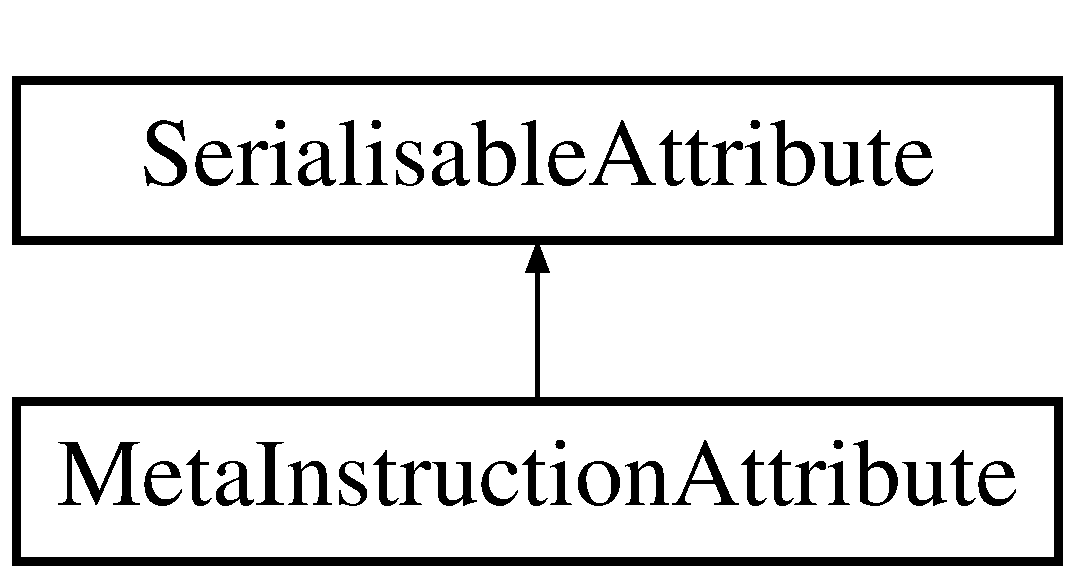
\includegraphics[height=2.000000cm]{classMetaInstructionAttribute}
\end{center}
\end{figure}
\subsection*{Public Member Functions}
\begin{DoxyCompactItemize}
\item 
\hyperlink{classMetaInstructionAttribute_a191d7f515a704ce03dd08bd70a99f505}{Meta\+Instruction\+Attribute} ()
\item 
\hyperlink{classMetaInstructionAttribute}{Meta\+Instruction\+Attribute} $\ast$ \hyperlink{classMetaInstructionAttribute_ae2650f9203c48687539dd550574937ba}{clone} ()
\item 
string \hyperlink{classMetaInstructionAttribute_a6f48798affab7135022b0a7d53c24430}{get\+Objdump\+Instr} ()
\item 
void \hyperlink{classMetaInstructionAttribute_a9fc979d829aaf9598c58a22f482ce134}{set\+Objdump\+Instr} (string vcode)
\item 
ostream \& \hyperlink{classMetaInstructionAttribute_a6b4f27589f0fc145ed4c23c5763f5930}{Write\+Xml} (std\+::ostream \&, cfglib\+::\+Handle \&)
\item 
void \hyperlink{classMetaInstructionAttribute_a5c2c96126868d18fac5828ce29285046}{Read\+Xml} (Xml\+Tag const $\ast$xml\+\_\+node, cfglib\+::\+Handle \&)
\item 
Serialisable\+Attribute $\ast$ \hyperlink{classMetaInstructionAttribute_a23e508c5ca9c295a510a69c9c5e942ba}{create} ()
\item 
void \hyperlink{classMetaInstructionAttribute_aadfd48ff5e2587e7535954acb6439a17}{Print} (std\+::ostream \&)
\end{DoxyCompactItemize}


\subsection{Constructor \& Destructor Documentation}
\mbox{\Hypertarget{classMetaInstructionAttribute_a191d7f515a704ce03dd08bd70a99f505}\label{classMetaInstructionAttribute_a191d7f515a704ce03dd08bd70a99f505}} 
\index{Meta\+Instruction\+Attribute@{Meta\+Instruction\+Attribute}!Meta\+Instruction\+Attribute@{Meta\+Instruction\+Attribute}}
\index{Meta\+Instruction\+Attribute@{Meta\+Instruction\+Attribute}!Meta\+Instruction\+Attribute@{Meta\+Instruction\+Attribute}}
\subsubsection{\texorpdfstring{Meta\+Instruction\+Attribute()}{MetaInstructionAttribute()}}
{\footnotesize\ttfamily Meta\+Instruction\+Attribute\+::\+Meta\+Instruction\+Attribute (\begin{DoxyParamCaption}{ }\end{DoxyParamCaption})}

constructor 

\subsection{Member Function Documentation}
\mbox{\Hypertarget{classMetaInstructionAttribute_ae2650f9203c48687539dd550574937ba}\label{classMetaInstructionAttribute_ae2650f9203c48687539dd550574937ba}} 
\index{Meta\+Instruction\+Attribute@{Meta\+Instruction\+Attribute}!clone@{clone}}
\index{clone@{clone}!Meta\+Instruction\+Attribute@{Meta\+Instruction\+Attribute}}
\subsubsection{\texorpdfstring{clone()}{clone()}}
{\footnotesize\ttfamily \hyperlink{classMetaInstructionAttribute}{Meta\+Instruction\+Attribute}$\ast$ Meta\+Instruction\+Attribute\+::clone (\begin{DoxyParamCaption}{ }\end{DoxyParamCaption})}

\mbox{\Hypertarget{classMetaInstructionAttribute_a23e508c5ca9c295a510a69c9c5e942ba}\label{classMetaInstructionAttribute_a23e508c5ca9c295a510a69c9c5e942ba}} 
\index{Meta\+Instruction\+Attribute@{Meta\+Instruction\+Attribute}!create@{create}}
\index{create@{create}!Meta\+Instruction\+Attribute@{Meta\+Instruction\+Attribute}}
\subsubsection{\texorpdfstring{create()}{create()}}
{\footnotesize\ttfamily Serialisable\+Attribute$\ast$ Meta\+Instruction\+Attribute\+::create (\begin{DoxyParamCaption}{ }\end{DoxyParamCaption})}

\mbox{\Hypertarget{classMetaInstructionAttribute_a6f48798affab7135022b0a7d53c24430}\label{classMetaInstructionAttribute_a6f48798affab7135022b0a7d53c24430}} 
\index{Meta\+Instruction\+Attribute@{Meta\+Instruction\+Attribute}!get\+Objdump\+Instr@{get\+Objdump\+Instr}}
\index{get\+Objdump\+Instr@{get\+Objdump\+Instr}!Meta\+Instruction\+Attribute@{Meta\+Instruction\+Attribute}}
\subsubsection{\texorpdfstring{get\+Objdump\+Instr()}{getObjdumpInstr()}}
{\footnotesize\ttfamily string Meta\+Instruction\+Attribute\+::get\+Objdump\+Instr (\begin{DoxyParamCaption}{ }\end{DoxyParamCaption})}

\mbox{\Hypertarget{classMetaInstructionAttribute_aadfd48ff5e2587e7535954acb6439a17}\label{classMetaInstructionAttribute_aadfd48ff5e2587e7535954acb6439a17}} 
\index{Meta\+Instruction\+Attribute@{Meta\+Instruction\+Attribute}!Print@{Print}}
\index{Print@{Print}!Meta\+Instruction\+Attribute@{Meta\+Instruction\+Attribute}}
\subsubsection{\texorpdfstring{Print()}{Print()}}
{\footnotesize\ttfamily void Meta\+Instruction\+Attribute\+::\+Print (\begin{DoxyParamCaption}\item[{std\+::ostream \&}]{ }\end{DoxyParamCaption})}

\mbox{\Hypertarget{classMetaInstructionAttribute_a5c2c96126868d18fac5828ce29285046}\label{classMetaInstructionAttribute_a5c2c96126868d18fac5828ce29285046}} 
\index{Meta\+Instruction\+Attribute@{Meta\+Instruction\+Attribute}!Read\+Xml@{Read\+Xml}}
\index{Read\+Xml@{Read\+Xml}!Meta\+Instruction\+Attribute@{Meta\+Instruction\+Attribute}}
\subsubsection{\texorpdfstring{Read\+Xml()}{ReadXml()}}
{\footnotesize\ttfamily void Meta\+Instruction\+Attribute\+::\+Read\+Xml (\begin{DoxyParamCaption}\item[{Xml\+Tag const $\ast$}]{xml\+\_\+node,  }\item[{cfglib\+::\+Handle \&}]{ }\end{DoxyParamCaption})}

\mbox{\Hypertarget{classMetaInstructionAttribute_a9fc979d829aaf9598c58a22f482ce134}\label{classMetaInstructionAttribute_a9fc979d829aaf9598c58a22f482ce134}} 
\index{Meta\+Instruction\+Attribute@{Meta\+Instruction\+Attribute}!set\+Objdump\+Instr@{set\+Objdump\+Instr}}
\index{set\+Objdump\+Instr@{set\+Objdump\+Instr}!Meta\+Instruction\+Attribute@{Meta\+Instruction\+Attribute}}
\subsubsection{\texorpdfstring{set\+Objdump\+Instr()}{setObjdumpInstr()}}
{\footnotesize\ttfamily void Meta\+Instruction\+Attribute\+::set\+Objdump\+Instr (\begin{DoxyParamCaption}\item[{string}]{vcode }\end{DoxyParamCaption})}

\mbox{\Hypertarget{classMetaInstructionAttribute_a6b4f27589f0fc145ed4c23c5763f5930}\label{classMetaInstructionAttribute_a6b4f27589f0fc145ed4c23c5763f5930}} 
\index{Meta\+Instruction\+Attribute@{Meta\+Instruction\+Attribute}!Write\+Xml@{Write\+Xml}}
\index{Write\+Xml@{Write\+Xml}!Meta\+Instruction\+Attribute@{Meta\+Instruction\+Attribute}}
\subsubsection{\texorpdfstring{Write\+Xml()}{WriteXml()}}
{\footnotesize\ttfamily ostream\& Meta\+Instruction\+Attribute\+::\+Write\+Xml (\begin{DoxyParamCaption}\item[{std\+::ostream \&}]{,  }\item[{cfglib\+::\+Handle \&}]{ }\end{DoxyParamCaption})}



The documentation for this class was generated from the following file\+:\begin{DoxyCompactItemize}
\item 
src/\hyperlink{MetaInstructionAttribute_8h}{Meta\+Instruction\+Attribute.\+h}\end{DoxyCompactItemize}

\hypertarget{classSymbolTableAttribute}{}\section{Symbol\+Table\+Attribute Class Reference}
\label{classSymbolTableAttribute}\index{Symbol\+Table\+Attribute@{Symbol\+Table\+Attribute}}


{\ttfamily \#include $<$Symbol\+Table\+Attribute.\+h$>$}

Inheritance diagram for Symbol\+Table\+Attribute\+:\begin{figure}[H]
\begin{center}
\leavevmode
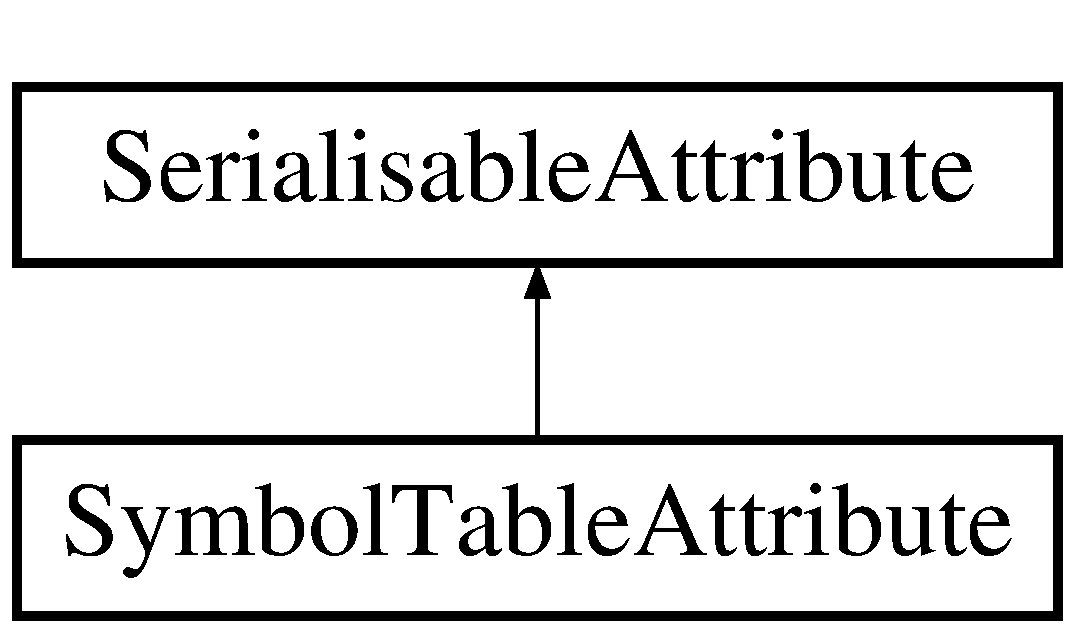
\includegraphics[height=2.000000cm]{classSymbolTableAttribute}
\end{center}
\end{figure}
\subsection*{Public Member Functions}
\begin{DoxyCompactItemize}
\item 
\hyperlink{classSymbolTableAttribute_a0540a38b6c87455ae69f989d45777cb7}{Symbol\+Table\+Attribute} ()
\item 
\hyperlink{classSymbolTableAttribute}{Symbol\+Table\+Attribute} $\ast$ \hyperlink{classSymbolTableAttribute_a0211a7147715180eb5cc7da65e72cf7d}{clone} ()
\item 
ostream \& \hyperlink{classSymbolTableAttribute_a8caf49a2a632b014a597acee79d3b4ce}{Write\+Xml} (std\+::ostream \&, cfglib\+::\+Handle \&)
\item 
void \hyperlink{classSymbolTableAttribute_ae3a962fbcb5eebcf2f5b9b25814d6714}{Read\+Xml} (Xml\+Tag const $\ast$xml\+\_\+node, cfglib\+::\+Handle \&)
\item 
Serialisable\+Attribute $\ast$ \hyperlink{classSymbolTableAttribute_aabc11b586cbe3f02b1d1b2838630fbb0}{create} ()
\item 
void \hyperlink{classSymbolTableAttribute_ab456077a4c556eec9ad24103689aa672}{Print} (std\+::ostream \&)
\item 
void \hyperlink{classSymbolTableAttribute_ac3d05fcd8b84f1b19e313ca35ab46b6a}{add\+Section} (std\+::string name, unsigned long addr, int size)
\item 
void \hyperlink{classSymbolTableAttribute_a37e4e5f0139566dfd77385ced03c1acb}{add\+Variable} (std\+::string name, unsigned long addr, int size, std\+::string section\+\_\+name)
\item 
void \hyperlink{classSymbolTableAttribute_a5cebeb90706d6570a12d4abd22ae0173}{set\+GP} (unsigned long val)
\item 
unsigned long \hyperlink{classSymbolTableAttribute_abb86ee2aeee7b78d4c93ee083fe7cdb6}{get\+GP} ()
\item 
unsigned long \hyperlink{classSymbolTableAttribute_a22e7e68ba19d0c9ea1d5ccfbe02336c2}{get\+Code\+Start\+Addr} ()
\item 
void \hyperlink{classSymbolTableAttribute_a6b87c838b987ba648eed8423323b5bf2}{get\+Info} (unsigned long addr, string $\ast$var\+\_\+name, unsigned long $\ast$start\+\_\+addr, int $\ast$size, string $\ast$section\+\_\+name)
\end{DoxyCompactItemize}


\subsection{Constructor \& Destructor Documentation}
\mbox{\Hypertarget{classSymbolTableAttribute_a0540a38b6c87455ae69f989d45777cb7}\label{classSymbolTableAttribute_a0540a38b6c87455ae69f989d45777cb7}} 
\index{Symbol\+Table\+Attribute@{Symbol\+Table\+Attribute}!Symbol\+Table\+Attribute@{Symbol\+Table\+Attribute}}
\index{Symbol\+Table\+Attribute@{Symbol\+Table\+Attribute}!Symbol\+Table\+Attribute@{Symbol\+Table\+Attribute}}
\subsubsection{\texorpdfstring{Symbol\+Table\+Attribute()}{SymbolTableAttribute()}}
{\footnotesize\ttfamily Symbol\+Table\+Attribute\+::\+Symbol\+Table\+Attribute (\begin{DoxyParamCaption}{ }\end{DoxyParamCaption})}

constructor 

\subsection{Member Function Documentation}
\mbox{\Hypertarget{classSymbolTableAttribute_ac3d05fcd8b84f1b19e313ca35ab46b6a}\label{classSymbolTableAttribute_ac3d05fcd8b84f1b19e313ca35ab46b6a}} 
\index{Symbol\+Table\+Attribute@{Symbol\+Table\+Attribute}!add\+Section@{add\+Section}}
\index{add\+Section@{add\+Section}!Symbol\+Table\+Attribute@{Symbol\+Table\+Attribute}}
\subsubsection{\texorpdfstring{add\+Section()}{addSection()}}
{\footnotesize\ttfamily void Symbol\+Table\+Attribute\+::add\+Section (\begin{DoxyParamCaption}\item[{std\+::string}]{name,  }\item[{unsigned long}]{addr,  }\item[{int}]{size }\end{DoxyParamCaption})}

\mbox{\Hypertarget{classSymbolTableAttribute_a37e4e5f0139566dfd77385ced03c1acb}\label{classSymbolTableAttribute_a37e4e5f0139566dfd77385ced03c1acb}} 
\index{Symbol\+Table\+Attribute@{Symbol\+Table\+Attribute}!add\+Variable@{add\+Variable}}
\index{add\+Variable@{add\+Variable}!Symbol\+Table\+Attribute@{Symbol\+Table\+Attribute}}
\subsubsection{\texorpdfstring{add\+Variable()}{addVariable()}}
{\footnotesize\ttfamily void Symbol\+Table\+Attribute\+::add\+Variable (\begin{DoxyParamCaption}\item[{std\+::string}]{name,  }\item[{unsigned long}]{addr,  }\item[{int}]{size,  }\item[{std\+::string}]{section\+\_\+name }\end{DoxyParamCaption})}

\mbox{\Hypertarget{classSymbolTableAttribute_a0211a7147715180eb5cc7da65e72cf7d}\label{classSymbolTableAttribute_a0211a7147715180eb5cc7da65e72cf7d}} 
\index{Symbol\+Table\+Attribute@{Symbol\+Table\+Attribute}!clone@{clone}}
\index{clone@{clone}!Symbol\+Table\+Attribute@{Symbol\+Table\+Attribute}}
\subsubsection{\texorpdfstring{clone()}{clone()}}
{\footnotesize\ttfamily \hyperlink{classSymbolTableAttribute}{Symbol\+Table\+Attribute}$\ast$ Symbol\+Table\+Attribute\+::clone (\begin{DoxyParamCaption}{ }\end{DoxyParamCaption})}

cloning function \mbox{\Hypertarget{classSymbolTableAttribute_aabc11b586cbe3f02b1d1b2838630fbb0}\label{classSymbolTableAttribute_aabc11b586cbe3f02b1d1b2838630fbb0}} 
\index{Symbol\+Table\+Attribute@{Symbol\+Table\+Attribute}!create@{create}}
\index{create@{create}!Symbol\+Table\+Attribute@{Symbol\+Table\+Attribute}}
\subsubsection{\texorpdfstring{create()}{create()}}
{\footnotesize\ttfamily Serialisable\+Attribute$\ast$ Symbol\+Table\+Attribute\+::create (\begin{DoxyParamCaption}{ }\end{DoxyParamCaption})}

\mbox{\Hypertarget{classSymbolTableAttribute_a22e7e68ba19d0c9ea1d5ccfbe02336c2}\label{classSymbolTableAttribute_a22e7e68ba19d0c9ea1d5ccfbe02336c2}} 
\index{Symbol\+Table\+Attribute@{Symbol\+Table\+Attribute}!get\+Code\+Start\+Addr@{get\+Code\+Start\+Addr}}
\index{get\+Code\+Start\+Addr@{get\+Code\+Start\+Addr}!Symbol\+Table\+Attribute@{Symbol\+Table\+Attribute}}
\subsubsection{\texorpdfstring{get\+Code\+Start\+Addr()}{getCodeStartAddr()}}
{\footnotesize\ttfamily unsigned long Symbol\+Table\+Attribute\+::get\+Code\+Start\+Addr (\begin{DoxyParamCaption}{ }\end{DoxyParamCaption})}

\mbox{\Hypertarget{classSymbolTableAttribute_abb86ee2aeee7b78d4c93ee083fe7cdb6}\label{classSymbolTableAttribute_abb86ee2aeee7b78d4c93ee083fe7cdb6}} 
\index{Symbol\+Table\+Attribute@{Symbol\+Table\+Attribute}!get\+GP@{get\+GP}}
\index{get\+GP@{get\+GP}!Symbol\+Table\+Attribute@{Symbol\+Table\+Attribute}}
\subsubsection{\texorpdfstring{get\+G\+P()}{getGP()}}
{\footnotesize\ttfamily unsigned long Symbol\+Table\+Attribute\+::get\+GP (\begin{DoxyParamCaption}{ }\end{DoxyParamCaption})}

\mbox{\Hypertarget{classSymbolTableAttribute_a6b87c838b987ba648eed8423323b5bf2}\label{classSymbolTableAttribute_a6b87c838b987ba648eed8423323b5bf2}} 
\index{Symbol\+Table\+Attribute@{Symbol\+Table\+Attribute}!get\+Info@{get\+Info}}
\index{get\+Info@{get\+Info}!Symbol\+Table\+Attribute@{Symbol\+Table\+Attribute}}
\subsubsection{\texorpdfstring{get\+Info()}{getInfo()}}
{\footnotesize\ttfamily void Symbol\+Table\+Attribute\+::get\+Info (\begin{DoxyParamCaption}\item[{unsigned long}]{addr,  }\item[{string $\ast$}]{var\+\_\+name,  }\item[{unsigned long $\ast$}]{start\+\_\+addr,  }\item[{int $\ast$}]{size,  }\item[{string $\ast$}]{section\+\_\+name }\end{DoxyParamCaption})}

Returns the informations\+: variable name, start\+\_\+addr, size and section name of the given addr. rq\+: the input address must be in decimal \mbox{\Hypertarget{classSymbolTableAttribute_ab456077a4c556eec9ad24103689aa672}\label{classSymbolTableAttribute_ab456077a4c556eec9ad24103689aa672}} 
\index{Symbol\+Table\+Attribute@{Symbol\+Table\+Attribute}!Print@{Print}}
\index{Print@{Print}!Symbol\+Table\+Attribute@{Symbol\+Table\+Attribute}}
\subsubsection{\texorpdfstring{Print()}{Print()}}
{\footnotesize\ttfamily void Symbol\+Table\+Attribute\+::\+Print (\begin{DoxyParamCaption}\item[{std\+::ostream \&}]{ }\end{DoxyParamCaption})}

\mbox{\Hypertarget{classSymbolTableAttribute_ae3a962fbcb5eebcf2f5b9b25814d6714}\label{classSymbolTableAttribute_ae3a962fbcb5eebcf2f5b9b25814d6714}} 
\index{Symbol\+Table\+Attribute@{Symbol\+Table\+Attribute}!Read\+Xml@{Read\+Xml}}
\index{Read\+Xml@{Read\+Xml}!Symbol\+Table\+Attribute@{Symbol\+Table\+Attribute}}
\subsubsection{\texorpdfstring{Read\+Xml()}{ReadXml()}}
{\footnotesize\ttfamily void Symbol\+Table\+Attribute\+::\+Read\+Xml (\begin{DoxyParamCaption}\item[{Xml\+Tag const $\ast$}]{xml\+\_\+node,  }\item[{cfglib\+::\+Handle \&}]{ }\end{DoxyParamCaption})}

\mbox{\Hypertarget{classSymbolTableAttribute_a5cebeb90706d6570a12d4abd22ae0173}\label{classSymbolTableAttribute_a5cebeb90706d6570a12d4abd22ae0173}} 
\index{Symbol\+Table\+Attribute@{Symbol\+Table\+Attribute}!set\+GP@{set\+GP}}
\index{set\+GP@{set\+GP}!Symbol\+Table\+Attribute@{Symbol\+Table\+Attribute}}
\subsubsection{\texorpdfstring{set\+G\+P()}{setGP()}}
{\footnotesize\ttfamily void Symbol\+Table\+Attribute\+::set\+GP (\begin{DoxyParamCaption}\item[{unsigned long}]{val }\end{DoxyParamCaption})}

\mbox{\Hypertarget{classSymbolTableAttribute_a8caf49a2a632b014a597acee79d3b4ce}\label{classSymbolTableAttribute_a8caf49a2a632b014a597acee79d3b4ce}} 
\index{Symbol\+Table\+Attribute@{Symbol\+Table\+Attribute}!Write\+Xml@{Write\+Xml}}
\index{Write\+Xml@{Write\+Xml}!Symbol\+Table\+Attribute@{Symbol\+Table\+Attribute}}
\subsubsection{\texorpdfstring{Write\+Xml()}{WriteXml()}}
{\footnotesize\ttfamily ostream\& Symbol\+Table\+Attribute\+::\+Write\+Xml (\begin{DoxyParamCaption}\item[{std\+::ostream \&}]{,  }\item[{cfglib\+::\+Handle \&}]{ }\end{DoxyParamCaption})}



The documentation for this class was generated from the following file\+:\begin{DoxyCompactItemize}
\item 
src/\hyperlink{SymbolTableAttribute_8h}{Symbol\+Table\+Attribute.\+h}\end{DoxyCompactItemize}

\hypertarget{classtriplet}{}\section{triplet Class Reference}
\label{classtriplet}\index{triplet@{triplet}}


{\ttfamily \#include $<$Symbol\+Table\+Attribute.\+h$>$}

\subsection*{Public Member Functions}
\begin{DoxyCompactItemize}
\item 
\hyperlink{classtriplet_a01cfe4002bbd14a8eaa841697bc3a336}{triplet} ()
\item 
\hyperlink{classtriplet_ab2d03159a2e99fee8d621dddec481d66}{triplet} (unsigned long v1, int v2, std\+::string v3)
\end{DoxyCompactItemize}
\subsection*{Public Attributes}
\begin{DoxyCompactItemize}
\item 
unsigned long \hyperlink{classtriplet_a3af8f9c37ea8230ec41a2e576f31cacd}{first}
\item 
int \hyperlink{classtriplet_ae2f96f25885f90f2668d142b31e9dac4}{second}
\item 
std\+::string \hyperlink{classtriplet_ab4d72eb35d165043734c7e870c01677f}{third}
\end{DoxyCompactItemize}


\subsection{Constructor \& Destructor Documentation}
\mbox{\Hypertarget{classtriplet_a01cfe4002bbd14a8eaa841697bc3a336}\label{classtriplet_a01cfe4002bbd14a8eaa841697bc3a336}} 
\index{triplet@{triplet}!triplet@{triplet}}
\index{triplet@{triplet}!triplet@{triplet}}
\subsubsection{\texorpdfstring{triplet()}{triplet()}\hspace{0.1cm}{\footnotesize\ttfamily [1/2]}}
{\footnotesize\ttfamily triplet\+::triplet (\begin{DoxyParamCaption}{ }\end{DoxyParamCaption})\hspace{0.3cm}{\ttfamily [inline]}}

\mbox{\Hypertarget{classtriplet_ab2d03159a2e99fee8d621dddec481d66}\label{classtriplet_ab2d03159a2e99fee8d621dddec481d66}} 
\index{triplet@{triplet}!triplet@{triplet}}
\index{triplet@{triplet}!triplet@{triplet}}
\subsubsection{\texorpdfstring{triplet()}{triplet()}\hspace{0.1cm}{\footnotesize\ttfamily [2/2]}}
{\footnotesize\ttfamily triplet\+::triplet (\begin{DoxyParamCaption}\item[{unsigned long}]{v1,  }\item[{int}]{v2,  }\item[{std\+::string}]{v3 }\end{DoxyParamCaption})\hspace{0.3cm}{\ttfamily [inline]}}



\subsection{Member Data Documentation}
\mbox{\Hypertarget{classtriplet_a3af8f9c37ea8230ec41a2e576f31cacd}\label{classtriplet_a3af8f9c37ea8230ec41a2e576f31cacd}} 
\index{triplet@{triplet}!first@{first}}
\index{first@{first}!triplet@{triplet}}
\subsubsection{\texorpdfstring{first}{first}}
{\footnotesize\ttfamily unsigned long triplet\+::first}

\mbox{\Hypertarget{classtriplet_ae2f96f25885f90f2668d142b31e9dac4}\label{classtriplet_ae2f96f25885f90f2668d142b31e9dac4}} 
\index{triplet@{triplet}!second@{second}}
\index{second@{second}!triplet@{triplet}}
\subsubsection{\texorpdfstring{second}{second}}
{\footnotesize\ttfamily int triplet\+::second}

\mbox{\Hypertarget{classtriplet_ab4d72eb35d165043734c7e870c01677f}\label{classtriplet_ab4d72eb35d165043734c7e870c01677f}} 
\index{triplet@{triplet}!third@{third}}
\index{third@{third}!triplet@{triplet}}
\subsubsection{\texorpdfstring{third}{third}}
{\footnotesize\ttfamily std\+::string triplet\+::third}



The documentation for this class was generated from the following file\+:\begin{DoxyCompactItemize}
\item 
src/\hyperlink{SymbolTableAttribute_8h}{Symbol\+Table\+Attribute.\+h}\end{DoxyCompactItemize}

\chapter{File Documentation}
\hypertarget{AddressAttribute_8h}{}\section{src/\+Address\+Attribute.h File Reference}
\label{AddressAttribute_8h}\index{src/\+Address\+Attribute.\+h@{src/\+Address\+Attribute.\+h}}
{\ttfamily \#include $<$utility$>$}\newline
{\ttfamily \#include $<$string$>$}\newline
{\ttfamily \#include $<$vector$>$}\newline
{\ttfamily \#include \char`\"{}Cfg\+Lib.\+h\char`\"{}}\newline
\subsection*{Classes}
\begin{DoxyCompactItemize}
\item 
class \hyperlink{classAddressInfo}{Address\+Info}
\item 
class \hyperlink{classAddressAttribute}{Address\+Attribute}
\end{DoxyCompactItemize}
\subsection*{Macros}
\begin{DoxyCompactItemize}
\item 
\#define \hyperlink{AddressAttribute_8h_a687daf243693727d22d6b12d0722a0c2}{A\+D\+D\+R\+E\+S\+S\+A\+T\+T\+R\+I\+B\+U\+TE}
\end{DoxyCompactItemize}


\subsection{Macro Definition Documentation}
\mbox{\Hypertarget{AddressAttribute_8h_a687daf243693727d22d6b12d0722a0c2}\label{AddressAttribute_8h_a687daf243693727d22d6b12d0722a0c2}} 
\index{Address\+Attribute.\+h@{Address\+Attribute.\+h}!A\+D\+D\+R\+E\+S\+S\+A\+T\+T\+R\+I\+B\+U\+TE@{A\+D\+D\+R\+E\+S\+S\+A\+T\+T\+R\+I\+B\+U\+TE}}
\index{A\+D\+D\+R\+E\+S\+S\+A\+T\+T\+R\+I\+B\+U\+TE@{A\+D\+D\+R\+E\+S\+S\+A\+T\+T\+R\+I\+B\+U\+TE}!Address\+Attribute.\+h@{Address\+Attribute.\+h}}
\subsubsection{\texorpdfstring{A\+D\+D\+R\+E\+S\+S\+A\+T\+T\+R\+I\+B\+U\+TE}{ADDRESSATTRIBUTE}}
{\footnotesize\ttfamily \#define A\+D\+D\+R\+E\+S\+S\+A\+T\+T\+R\+I\+B\+U\+TE}


\hypertarget{ARMWordsAttribute_8h}{}\section{src/\+A\+R\+M\+Words\+Attribute.h File Reference}
\label{ARMWordsAttribute_8h}\index{src/\+A\+R\+M\+Words\+Attribute.\+h@{src/\+A\+R\+M\+Words\+Attribute.\+h}}
{\ttfamily \#include $<$utility$>$}\newline
{\ttfamily \#include $<$string$>$}\newline
{\ttfamily \#include $<$map$>$}\newline
{\ttfamily \#include \char`\"{}Cfg\+Lib.\+h\char`\"{}}\newline
\subsection*{Classes}
\begin{DoxyCompactItemize}
\item 
class \hyperlink{classARMWordsAttribute}{A\+R\+M\+Words\+Attribute}
\end{DoxyCompactItemize}
\subsection*{Typedefs}
\begin{DoxyCompactItemize}
\item 
typedef pair$<$ string, unsigned long $>$ \hyperlink{ARMWordsAttribute_8h_a95eba34e7dc7ec27245bdf7b054f43ae}{A\+R\+M\+Words\+Attribute\+Elem\+Table\+Value}
\item 
typedef map$<$ unsigned long, \hyperlink{ARMWordsAttribute_8h_a95eba34e7dc7ec27245bdf7b054f43ae}{A\+R\+M\+Words\+Attribute\+Elem\+Table\+Value} $>$ \hyperlink{ARMWordsAttribute_8h_a7d589468d1898466a80161546d217fd6}{A\+R\+M\+Words\+Attribute\+Table}
\end{DoxyCompactItemize}


\subsection{Typedef Documentation}
\mbox{\Hypertarget{ARMWordsAttribute_8h_a95eba34e7dc7ec27245bdf7b054f43ae}\label{ARMWordsAttribute_8h_a95eba34e7dc7ec27245bdf7b054f43ae}} 
\index{A\+R\+M\+Words\+Attribute.\+h@{A\+R\+M\+Words\+Attribute.\+h}!A\+R\+M\+Words\+Attribute\+Elem\+Table\+Value@{A\+R\+M\+Words\+Attribute\+Elem\+Table\+Value}}
\index{A\+R\+M\+Words\+Attribute\+Elem\+Table\+Value@{A\+R\+M\+Words\+Attribute\+Elem\+Table\+Value}!A\+R\+M\+Words\+Attribute.\+h@{A\+R\+M\+Words\+Attribute.\+h}}
\subsubsection{\texorpdfstring{A\+R\+M\+Words\+Attribute\+Elem\+Table\+Value}{ARMWordsAttributeElemTableValue}}
{\footnotesize\ttfamily typedef pair$<$ string, unsigned long$>$ \hyperlink{ARMWordsAttribute_8h_a95eba34e7dc7ec27245bdf7b054f43ae}{A\+R\+M\+Words\+Attribute\+Elem\+Table\+Value}}

\mbox{\Hypertarget{ARMWordsAttribute_8h_a7d589468d1898466a80161546d217fd6}\label{ARMWordsAttribute_8h_a7d589468d1898466a80161546d217fd6}} 
\index{A\+R\+M\+Words\+Attribute.\+h@{A\+R\+M\+Words\+Attribute.\+h}!A\+R\+M\+Words\+Attribute\+Table@{A\+R\+M\+Words\+Attribute\+Table}}
\index{A\+R\+M\+Words\+Attribute\+Table@{A\+R\+M\+Words\+Attribute\+Table}!A\+R\+M\+Words\+Attribute.\+h@{A\+R\+M\+Words\+Attribute.\+h}}
\subsubsection{\texorpdfstring{A\+R\+M\+Words\+Attribute\+Table}{ARMWordsAttributeTable}}
{\footnotesize\ttfamily typedef map$<$unsigned long, \hyperlink{ARMWordsAttribute_8h_a95eba34e7dc7ec27245bdf7b054f43ae}{A\+R\+M\+Words\+Attribute\+Elem\+Table\+Value} $>$ \hyperlink{ARMWordsAttribute_8h_a7d589468d1898466a80161546d217fd6}{A\+R\+M\+Words\+Attribute\+Table}}


\hypertarget{GlobalAttributes_8h}{}\section{src/\+Global\+Attributes.h File Reference}
\label{GlobalAttributes_8h}\index{src/\+Global\+Attributes.\+h@{src/\+Global\+Attributes.\+h}}
{\ttfamily \#include \char`\"{}Address\+Attribute.\+h\char`\"{}}\newline
{\ttfamily \#include \char`\"{}Symbol\+Table\+Attribute.\+h\char`\"{}}\newline
{\ttfamily \#include \char`\"{}A\+R\+M\+Words\+Attribute.\+h\char`\"{}}\newline
{\ttfamily \#include \char`\"{}Meta\+Instruction\+Attribute.\+h\char`\"{}}\newline
\subsection*{Macros}
\begin{DoxyCompactItemize}
\item 
\#define \hyperlink{GlobalAttributes_8h_ad44d99c7b3f7475bd218df9404f87c03}{Maxiter\+Attribute\+Name}~\char`\"{}maxiter\char`\"{}
\item 
\#define \hyperlink{GlobalAttributes_8h_ad9d9e2f565d56ad74106811524c56fbf}{Address\+Attribute\+Name}~\char`\"{}address\char`\"{}
\item 
\#define \hyperlink{GlobalAttributes_8h_aee8be085ade601db6d0dd816157b9a16}{Symbol\+Table\+Attribute\+Name}~\char`\"{}symbol\+Table\char`\"{}
\item 
\#define \hyperlink{GlobalAttributes_8h_a77bdc1fe342840a91d0dec31b5594652}{A\+R\+M\+Words\+Attribute\+Name}~\char`\"{}A\+R\+M\+\_\+\+W\+O\+R\+DS\char`\"{}
\item 
\#define \hyperlink{GlobalAttributes_8h_af75af298a4300f96f696661844cb5667}{Meta\+Instruction\+Attribute\+Name}~\char`\"{}Meta\+Instruction\char`\"{}
\end{DoxyCompactItemize}


\subsection{Macro Definition Documentation}
\mbox{\Hypertarget{GlobalAttributes_8h_ad9d9e2f565d56ad74106811524c56fbf}\label{GlobalAttributes_8h_ad9d9e2f565d56ad74106811524c56fbf}} 
\index{Global\+Attributes.\+h@{Global\+Attributes.\+h}!Address\+Attribute\+Name@{Address\+Attribute\+Name}}
\index{Address\+Attribute\+Name@{Address\+Attribute\+Name}!Global\+Attributes.\+h@{Global\+Attributes.\+h}}
\subsubsection{\texorpdfstring{Address\+Attribute\+Name}{AddressAttributeName}}
{\footnotesize\ttfamily \#define Address\+Attribute\+Name~\char`\"{}address\char`\"{}}

\mbox{\Hypertarget{GlobalAttributes_8h_a77bdc1fe342840a91d0dec31b5594652}\label{GlobalAttributes_8h_a77bdc1fe342840a91d0dec31b5594652}} 
\index{Global\+Attributes.\+h@{Global\+Attributes.\+h}!A\+R\+M\+Words\+Attribute\+Name@{A\+R\+M\+Words\+Attribute\+Name}}
\index{A\+R\+M\+Words\+Attribute\+Name@{A\+R\+M\+Words\+Attribute\+Name}!Global\+Attributes.\+h@{Global\+Attributes.\+h}}
\subsubsection{\texorpdfstring{A\+R\+M\+Words\+Attribute\+Name}{ARMWordsAttributeName}}
{\footnotesize\ttfamily \#define A\+R\+M\+Words\+Attribute\+Name~\char`\"{}A\+R\+M\+\_\+\+W\+O\+R\+DS\char`\"{}}

\mbox{\Hypertarget{GlobalAttributes_8h_ad44d99c7b3f7475bd218df9404f87c03}\label{GlobalAttributes_8h_ad44d99c7b3f7475bd218df9404f87c03}} 
\index{Global\+Attributes.\+h@{Global\+Attributes.\+h}!Maxiter\+Attribute\+Name@{Maxiter\+Attribute\+Name}}
\index{Maxiter\+Attribute\+Name@{Maxiter\+Attribute\+Name}!Global\+Attributes.\+h@{Global\+Attributes.\+h}}
\subsubsection{\texorpdfstring{Maxiter\+Attribute\+Name}{MaxiterAttributeName}}
{\footnotesize\ttfamily \#define Maxiter\+Attribute\+Name~\char`\"{}maxiter\char`\"{}}

\subsubsection*{Loop bound attribute }

Maximum number of iterations for loops This attribute is set by the C\+FG extractor (annotations embedded in source code or external xml file) and is retrieved by any subsequent analysis step \mbox{\Hypertarget{GlobalAttributes_8h_af75af298a4300f96f696661844cb5667}\label{GlobalAttributes_8h_af75af298a4300f96f696661844cb5667}} 
\index{Global\+Attributes.\+h@{Global\+Attributes.\+h}!Meta\+Instruction\+Attribute\+Name@{Meta\+Instruction\+Attribute\+Name}}
\index{Meta\+Instruction\+Attribute\+Name@{Meta\+Instruction\+Attribute\+Name}!Global\+Attributes.\+h@{Global\+Attributes.\+h}}
\subsubsection{\texorpdfstring{Meta\+Instruction\+Attribute\+Name}{MetaInstructionAttributeName}}
{\footnotesize\ttfamily \#define Meta\+Instruction\+Attribute\+Name~\char`\"{}Meta\+Instruction\char`\"{}}

Attached to A\+RM to added instruction for the translation of pusp, pop, ldm, stm instructions. Attached by the C\+FG extractor \mbox{\Hypertarget{GlobalAttributes_8h_aee8be085ade601db6d0dd816157b9a16}\label{GlobalAttributes_8h_aee8be085ade601db6d0dd816157b9a16}} 
\index{Global\+Attributes.\+h@{Global\+Attributes.\+h}!Symbol\+Table\+Attribute\+Name@{Symbol\+Table\+Attribute\+Name}}
\index{Symbol\+Table\+Attribute\+Name@{Symbol\+Table\+Attribute\+Name}!Global\+Attributes.\+h@{Global\+Attributes.\+h}}
\subsubsection{\texorpdfstring{Symbol\+Table\+Attribute\+Name}{SymbolTableAttributeName}}
{\footnotesize\ttfamily \#define Symbol\+Table\+Attribute\+Name~\char`\"{}symbol\+Table\char`\"{}}


\hypertarget{LoopTree_8h}{}\section{src/\+Loop\+Tree.h File Reference}
\label{LoopTree_8h}\index{src/\+Loop\+Tree.\+h@{src/\+Loop\+Tree.\+h}}
{\ttfamily \#include $<$assert.\+h$>$}\newline
{\ttfamily \#include \char`\"{}Loop.\+h\char`\"{}}\newline
{\ttfamily \#include \char`\"{}Program.\+h\char`\"{}}\newline
{\ttfamily \#include \char`\"{}Node.\+h\char`\"{}}\newline
{\ttfamily \#include \char`\"{}Cfg.\+h\char`\"{}}\newline
{\ttfamily \#include \char`\"{}Helper.\+h\char`\"{}}\newline
\subsection*{Classes}
\begin{DoxyCompactItemize}
\item 
class \hyperlink{classLoopTreeNode}{Loop\+Tree\+Node}
\item 
class \hyperlink{classLoopTree}{Loop\+Tree}
\end{DoxyCompactItemize}

\hypertarget{MetaInstructionAttribute_8h}{}\section{src/\+Meta\+Instruction\+Attribute.h File Reference}
\label{MetaInstructionAttribute_8h}\index{src/\+Meta\+Instruction\+Attribute.\+h@{src/\+Meta\+Instruction\+Attribute.\+h}}
{\ttfamily \#include $<$utility$>$}\newline
{\ttfamily \#include $<$string$>$}\newline
{\ttfamily \#include $<$map$>$}\newline
{\ttfamily \#include \char`\"{}Cfg\+Lib.\+h\char`\"{}}\newline
\subsection*{Classes}
\begin{DoxyCompactItemize}
\item 
class \hyperlink{classMetaInstructionAttribute}{Meta\+Instruction\+Attribute}
\end{DoxyCompactItemize}

\hypertarget{SymbolTableAttribute_8h}{}\section{src/\+Symbol\+Table\+Attribute.h File Reference}
\label{SymbolTableAttribute_8h}\index{src/\+Symbol\+Table\+Attribute.\+h@{src/\+Symbol\+Table\+Attribute.\+h}}
{\ttfamily \#include $<$string$>$}\newline
{\ttfamily \#include $<$utility$>$}\newline
{\ttfamily \#include $<$map$>$}\newline
{\ttfamily \#include \char`\"{}Cfg\+Lib.\+h\char`\"{}}\newline
\subsection*{Classes}
\begin{DoxyCompactItemize}
\item 
class \hyperlink{classtriplet}{triplet}
\item 
class \hyperlink{classSymbolTableAttribute}{Symbol\+Table\+Attribute}
\end{DoxyCompactItemize}

%--- End generated contents ---

% Index
\backmatter
\newpage
\phantomsection
\clearemptydoublepage
\addcontentsline{toc}{chapter}{Index}
\printindex

\end{document}
